\documentclass[twoside]{book}

% Packages required by doxygen
\usepackage{fixltx2e}
\usepackage{calc}
\usepackage{doxygen}
\usepackage[export]{adjustbox} % also loads graphicx
\usepackage{graphicx}
\usepackage[utf8]{inputenc}
\usepackage{makeidx}
\usepackage{multicol}
\usepackage{multirow}
\PassOptionsToPackage{warn}{textcomp}
\usepackage{textcomp}
\usepackage[nointegrals]{wasysym}
\usepackage[table]{xcolor}

% Font selection
\usepackage[T1]{fontenc}
\usepackage[scaled=.90]{helvet}
\usepackage{courier}
\usepackage{amssymb}
\usepackage{sectsty}
\renewcommand{\familydefault}{\sfdefault}
\allsectionsfont{%
  \fontseries{bc}\selectfont%
  \color{darkgray}%
}
\renewcommand{\DoxyLabelFont}{%
  \fontseries{bc}\selectfont%
  \color{darkgray}%
}
\newcommand{\+}{\discretionary{\mbox{\scriptsize$\hookleftarrow$}}{}{}}

% Page & text layout
\usepackage{geometry}
\geometry{%
  a4paper,%
  top=2.5cm,%
  bottom=2.5cm,%
  left=2.5cm,%
  right=2.5cm%
}
\tolerance=750
\hfuzz=15pt
\hbadness=750
\setlength{\emergencystretch}{15pt}
\setlength{\parindent}{0cm}
\setlength{\parskip}{3ex plus 2ex minus 2ex}
\makeatletter
\renewcommand{\paragraph}{%
  \@startsection{paragraph}{4}{0ex}{-1.0ex}{1.0ex}{%
    \normalfont\normalsize\bfseries\SS@parafont%
  }%
}
\renewcommand{\subparagraph}{%
  \@startsection{subparagraph}{5}{0ex}{-1.0ex}{1.0ex}{%
    \normalfont\normalsize\bfseries\SS@subparafont%
  }%
}
\makeatother

% Headers & footers
\usepackage{fancyhdr}
\pagestyle{fancyplain}
\fancyhead[LE]{\fancyplain{}{\bfseries\thepage}}
\fancyhead[CE]{\fancyplain{}{}}
\fancyhead[RE]{\fancyplain{}{\bfseries\leftmark}}
\fancyhead[LO]{\fancyplain{}{\bfseries\rightmark}}
\fancyhead[CO]{\fancyplain{}{}}
\fancyhead[RO]{\fancyplain{}{\bfseries\thepage}}
\fancyfoot[LE]{\fancyplain{}{}}
\fancyfoot[CE]{\fancyplain{}{}}
\fancyfoot[RE]{\fancyplain{}{\bfseries\scriptsize Generated by Doxygen }}
\fancyfoot[LO]{\fancyplain{}{\bfseries\scriptsize Generated by Doxygen }}
\fancyfoot[CO]{\fancyplain{}{}}
\fancyfoot[RO]{\fancyplain{}{}}
\renewcommand{\footrulewidth}{0.4pt}
\renewcommand{\chaptermark}[1]{%
  \markboth{#1}{}%
}
\renewcommand{\sectionmark}[1]{%
  \markright{\thesection\ #1}%
}

% Indices & bibliography
\usepackage{natbib}
\usepackage[titles]{tocloft}
\setcounter{tocdepth}{3}
\setcounter{secnumdepth}{5}
\makeindex

% Hyperlinks (required, but should be loaded last)
\usepackage{ifpdf}
\ifpdf
  \usepackage[pdftex,pagebackref=true]{hyperref}
\else
  \usepackage[ps2pdf,pagebackref=true]{hyperref}
\fi
\hypersetup{%
  colorlinks=true,%
  linkcolor=blue,%
  citecolor=blue,%
  unicode%
}

% Custom commands
\newcommand{\clearemptydoublepage}{%
  \newpage{\pagestyle{empty}\cleardoublepage}%
}

\usepackage{caption}
\captionsetup{labelsep=space,justification=centering,font={bf},singlelinecheck=off,skip=4pt,position=top}

%===== C O N T E N T S =====

\begin{document}

% Titlepage & ToC
\hypersetup{pageanchor=false,
             bookmarksnumbered=true,
             pdfencoding=unicode
            }
\pagenumbering{alph}
\begin{titlepage}
\vspace*{7cm}
\begin{center}%
{\Large C++ Arg\+Parse }\\
\vspace*{1cm}
{\large Generated by Doxygen 1.8.13}\\
\end{center}
\end{titlepage}
\clearemptydoublepage
\pagenumbering{roman}
\tableofcontents
\clearemptydoublepage
\pagenumbering{arabic}
\hypersetup{pageanchor=true}

%--- Begin generated contents ---
\chapter{C++ Arg\+Parse\+: command line parsing made simple}
\label{index}\hypertarget{index}{}This is the source code documentation for C++ Arg\+Parse. 
\chapter{C++ Arg\+Parse\+: command line parsing made simple}
\label{md_README}
\Hypertarget{md_README}
C++ Arg\+Parse is an open source header-\/only C++11 library for parsing the command line ({\ttfamily argc}, {\ttfamily argv}) in a typed manner.

Due to the core\textquotesingle{}s heavy usage of template magic, the library can expose a very easy-\/to-\/use interface, so you as an application developer only have to care about the good stuff. Think Python\textquotesingle{}s \href{https://docs.python.org/3/library/argparse.html}{\tt argparse}.

\href{https://travis-ci.org/backraw/cppargparse}{\tt }

The source code documentation and code coverage results can be found here\+: \href{https://backraw.github.io/cppargparse}{\tt https\+://backraw.\+github.\+io/cppargparse}

\section*{Build tests}

Build requirements\+:
\begin{DoxyItemize}
\item {\ttfamily gcc}, {\ttfamily clang}, or {\ttfamily msvc}
\item {\ttfamily cmake}
\end{DoxyItemize}

\#\# Linux 
\begin{DoxyCode}
git clone https://github.com/backraw/cppargparse.git
cd cppargparse

mkdir build
cd build

cmake -DCMAKE\_BUILD\_TYPE=Profiling ..
make run\_tests
\end{DoxyCode}


Of course, you can use every generator that C\+Make supports like Ninja, etc.

\subsection*{Windows}


\begin{DoxyItemize}
\item Create the {\ttfamily build} directory inside the project directory
\item Run {\ttfamily cmake -\/G\char`\"{}\+Visual Studio 14 Win64\char`\"{} -\/\+D\+C\+M\+A\+K\+E\+\_\+\+B\+U\+I\+L\+D\+\_\+\+T\+Y\+PE=Debug ..}
\item Open {\ttfamily cppargparse.\+sln}
\item Build {\ttfamily R\+U\+N\+\_\+\+T\+E\+S\+TS}
\end{DoxyItemize}

{\itshape Requires at least Visual Studio 2015. This is because of G\+Test, which cannot be compiled using Visual Studio 2013 (A\+F\+A\+IK).}

Or simply use Min\+GW and do it the Linux way on Windows.

\section*{Code coverage}

Coverage requirements\+:
\begin{DoxyItemize}
\item {\ttfamily gcov}
\item {\ttfamily lcov}
\item {\ttfamily genhtml}
\item {\ttfamily python3}
\end{DoxyItemize}

Run {\ttfamily make coverage} inside the build directory. This will automatically execute {\ttfamily make run\+\_\+tests} beforehand.

\section*{Install}

To install the library, run {\ttfamily sudo make install} inside the build directory.

\section*{The library interface}

Please have a look at the \href{https://github.com/backraw/cppargparse/tree/master/samples}{\tt examples}.

You can mix \href{https://github.com/backraw/cppargparse/tree/master/samples/traditional}{\tt traditional} and \href{https://github.com/backraw/cppargparse/tree/master/samples/callback}{\tt callback} arguments as you wish. The \href{https://github.com/backraw/cppargparse/blob/master/include/cppargparse/parser.h#L242}{\tt Argument\+Parser} class provides an interface for both and doesn\textquotesingle{}t care which one you chose.

\section*{The core}

All the magic is done via the typed {\ttfamily \hyperlink{structcppargparse_1_1argument}{cppargparse\+::argument}} struct. Each such struct definition {\bfseries must provide 3 static methods}\+:
\begin{DoxyItemize}
\item {\ttfamily T parse(cmd, position, cmdargs)}
\item {\ttfamily T convert(cmd, position, cmdargs)}
\item {\ttfamily const char $\ast$error\+\_\+string(position)}
\end{DoxyItemize}

Parameter definition\+:
\begin{DoxyItemize}
\item {\ttfamily cmd} represents the whole command line inside a {\ttfamily std\+::vector$<$std\+::string$>$}
\item {\ttfamily position} represents the argument iterator position inside {\ttfamily cmd}
\item {\ttfamily cmdargs} represents the \href{https://github.com/backraw/cppargparse/blob/master/include/cppargparse/types.h#L41}{\tt command line argument struct object}
\end{DoxyItemize}

The \href{https://github.com/backraw/cppargparse/blob/master/include/cppargparse/parser.h#L242}{\tt Argument\+Parser} class provides the {\ttfamily get\+\_\+option$<$T$>$(cmdarg)}, {\ttfamily get\+\_\+option$<$T$>$(cmdarg, default)} and {\ttfamily get\+\_\+flag(cmdarg)} methods for calling the actual type converter methods provided by the {\ttfamily \hyperlink{structcppargparse_1_1argument}{cppargparse\+::argument}$<$T$>$} structs.

Assume the following command line arguments have been passed\+: {\ttfamily -\/t 3 -\/n \char`\"{}\+My Name\char`\"{} -\/-\/enable} 
\begin{DoxyCode}
\{C++\}
// -t 3
parse<int>(<cmd>, <argument iterator position 0>, <cmdargs>)
// calls and returns the value of
convert<int>(<cmd>, <argument iterator position 1>, <cmdargs>)
// which is the integer 3.


// -n "My Name"
parse<std::string>(<cmd>, <argument iterator position 2>, <cmdargs>)
// calls and returns the value of
convert<std::string>(<cmd>, <argument iterator position 3>, <cmdargs>)
// which is the string "My Name".


// --enable
// flags are checked only for their existence inside <cmd>,
// they don't provide any conversion methods.
\end{DoxyCode}


\subsection*{Primitive numerical types}

Let\textquotesingle{}s look at the {\ttfamily int} type, for example\+: 
\begin{DoxyCode}
\{C++\}
template <>
struct argument<int>
\{
    static int parse(cmd, position, cmdargs)
    \{
        return numerical\_argument<int>::convert(cmd, std::next(position), &wrap, "int");
    \}

    static int convert(cmd, position, cmdargs)
    \{
        return numerical\_argument<int>::convert(cmd, position, &wrap, "int");
    \}

    static int wrap(const std::string &s)
    \{
        return std::stoi(s);
    \}
\};
\end{DoxyCode}


All it does is the following\+:
\begin{DoxyItemize}
\item Call {\ttfamily cppargparse\+::numerical\+\_\+argument\+::parse$<$int$>$()} (or {\ttfamily convert$<$int$>$()}) on a command line argument iterator position {\ttfamily position}
\item Tell it to use {\ttfamily \hyperlink{structcppargparse_1_1argument}{cppargparse\+::argument}$<$int$>$\+::wrap()} as the conversion function
\end{DoxyItemize}

{\ttfamily wrap()} is needed, because {\ttfamily std\+::stoi()} (in the case of {\ttfamily int}) cannot be passed as a parameter, since it contains default parameters. {\ttfamily wrap()} just gets rid of them and makes the function \char`\"{}passable\char`\"{}.

The {\ttfamily \hyperlink{structcppargparse_1_1numerical__argument}{cppargparse\+::numerical\+\_\+argument}} struct wraps the actual convert-\/or-\/error mechanism\+: 
\begin{DoxyCode}
\{C++\}
template <typename T>
struct numerical\_argument
\{
    static T convert(cmd, position, numerical\_converter, type\_string)
    \{
        if (position == cmd.cend())
        \{
            throw errors::CommandLineOptionError(...)
        \}

        try
        \{
            return numerical\_converter(*position);
        \}

        catch (const std::invalid\_argument &)
        \{
            throw errors::CommandLineOptionError(...)
        \}
        catch (const std::out\_of\_range &)
        \{
            throw errors::CommandLineOptionError(...)
        \}
    \}

    static const std::string error\_message(position, type\_string)
    \{
        ...
    \}
\}
\end{DoxyCode}


{\ttfamily \hyperlink{structcppargparse_1_1numerical__argument_ab775dbbfc851bbd9052b70dfdf0dbb77}{cppargparse\+::numerical\+\_\+argument\+::convert()}} calls {\ttfamily numerical\+\_\+converter} with a string as the argument. {\ttfamily numerical\+\_\+converter} can (currently) be one of the following\+:

\tabulinesep=1mm
\begin{longtabu} spread 0pt [c]{*{3}{|X[-1]}|}
\hline
\rowcolor{\tableheadbgcolor}\textbf{ $\ast$$\ast$\+Data type$\ast$$\ast$}&\textbf{ $\ast$$\ast$\+Wrapped converter function$\ast$$\ast$}&\textbf{ C++ Arg\+Parse implementation  }\\\cline{1-3}
\endfirsthead
\hline
\endfoot
\hline
\rowcolor{\tableheadbgcolor}\textbf{ $\ast$$\ast$\+Data type$\ast$$\ast$}&\textbf{ $\ast$$\ast$\+Wrapped converter function$\ast$$\ast$}&\textbf{ C++ Arg\+Parse implementation  }\\\cline{1-3}
\endhead
{\ttfamily int}&{\ttfamily std\+::stoi}&\href{https://github.com/backraw/cppargparse/tree/master/include/cppargparse/arguments/int.h}{\tt int.\+h} \\\cline{1-3}
{\ttfamily unsigned int}&{\ttfamily stou} (custom implementation)&\href{https://github.com/backraw/cppargparse/tree/master/include/cppargparse/arguments/int.h}{\tt int.\+h} \\\cline{1-3}
{\ttfamily long}&{\ttfamily std\+::stol}&\href{https://github.com/backraw/cppargparse/tree/master/include/cppargparse/arguments/long.h}{\tt long.\+h} \\\cline{1-3}
{\ttfamily long long}&{\ttfamily std\+::stoll}&\href{https://github.com/backraw/cppargparse/tree/master/include/cppargparse/arguments/long.h}{\tt long.\+h} \\\cline{1-3}
{\ttfamily unsigned long}&{\ttfamily std\+::stoul}&\href{https://github.com/backraw/cppargparse/tree/master/include/cppargparse/arguments/long.h}{\tt long.\+h} \\\cline{1-3}
{\ttfamily unsigned long long}&{\ttfamily std\+::stoull}&\href{https://github.com/backraw/cppargparse/tree/master/include/cppargparse/arguments/long.h}{\tt long.\+h} \\\cline{1-3}
{\ttfamily float}&{\ttfamily std\+::stof}&\href{https://github.com/backraw/cppargparse/tree/master/include/cppargparse/arguments/float.h}{\tt float.\+h} \\\cline{1-3}
{\ttfamily double}&{\ttfamily std\+::stod}&\href{https://github.com/backraw/cppargparse/tree/master/include/cppargparse/arguments/long.h}{\tt double.\+h} \\\cline{1-3}
{\ttfamily long double}&{\ttfamily std\+::stold}&\href{https://github.com/backraw/cppargparse/tree/master/include/cppargparse/arguments/double.h}{\tt double.\+h} \\\cline{1-3}
\end{longtabu}


\subsection*{String types}

Currently only {\ttfamily std\+::string} is implemented as a string type\+: 
\begin{DoxyCode}
\{C++\}
static const std::string convert(cmd, position, cmdargs)
\{
    if (position == cmd.cend())
    \{
        throw errors::CommandLineOptionError(...);
    \}

    return *position;
\}
\end{DoxyCode}


It just checks whether the end of the command line argumnents list has been reached. If so, thrown an error, if not, return the string value for {\ttfamily position}.

\subsection*{Vector types}

Currently only {\ttfamily std\+::vector$<$T$>$} is implemented as a vector type\+: 
\begin{DoxyCode}
\{C++\}
template <typename T>
struct argument<std::vector<T>>
\{
    static const std::vector<T> parse(cmd, position, cmdargs)
    \{
        auto positions = get\_option\_positions(cmd, position, cmdargs);
        std::vector<T> values;

        for (auto position : positions)
        \{
            // Use the underlying argument::convert() method and store the returned value
            values.emplace\_back(argument<T>::convert(cmd, position, cmdargs));
        \}

        return values;
    \}


    static types::CommandLinePositions\_t get\_option\_positions(cmd, position, cmdargs)
    \{
        types::CommandLinePositions\_t positions;

        for (auto current = std::next(position); current != cmd.end(); ++current)
        \{
            if (algorithm::find\_arg(cmdargs, *current) != cmdargs.cend())
            \{
                break;
            \}

            positions.emplace\_back(current);
        \}

        return positions;
    \}
\}
\end{DoxyCode}


It collects all values tied to the argument and converts each value string to {\ttfamily T}.

\subsection*{Custom types}

... todo ... 
\chapter{Hierarchical Index}
\section{Class Hierarchy}
This inheritance list is sorted roughly, but not completely, alphabetically\+:\begin{DoxyCompactList}
\item \contentsline{section}{cppargparse\+:\+:argument$<$ T $>$}{\pageref{structcppargparse_1_1argument}}{}
\item \contentsline{section}{cppargparse\+:\+:argument$<$ double $>$}{\pageref{structcppargparse_1_1argument_3_01double_01_4}}{}
\item \contentsline{section}{cppargparse\+:\+:argument$<$ float $>$}{\pageref{structcppargparse_1_1argument_3_01float_01_4}}{}
\item \contentsline{section}{cppargparse\+:\+:argument$<$ int $>$}{\pageref{structcppargparse_1_1argument_3_01int_01_4}}{}
\item \contentsline{section}{cppargparse\+:\+:argument$<$ long $>$}{\pageref{structcppargparse_1_1argument_3_01long_01_4}}{}
\item \contentsline{section}{cppargparse\+:\+:argument$<$ long double $>$}{\pageref{structcppargparse_1_1argument_3_01long_01double_01_4}}{}
\item \contentsline{section}{cppargparse\+:\+:argument$<$ long long $>$}{\pageref{structcppargparse_1_1argument_3_01long_01long_01_4}}{}
\item \contentsline{section}{cppargparse\+:\+:argument$<$ std\+:\+:string $>$}{\pageref{structcppargparse_1_1argument_3_01std_1_1string_01_4}}{}
\item \contentsline{section}{cppargparse\+:\+:argument$<$ std\+:\+:vector$<$ T $>$ $>$}{\pageref{structcppargparse_1_1argument_3_01std_1_1vector_3_01T_01_4_01_4}}{}
\item \contentsline{section}{cppargparse\+:\+:argument$<$ unsigned int $>$}{\pageref{structcppargparse_1_1argument_3_01unsigned_01int_01_4}}{}
\item \contentsline{section}{cppargparse\+:\+:argument$<$ unsigned long $>$}{\pageref{structcppargparse_1_1argument_3_01unsigned_01long_01_4}}{}
\item \contentsline{section}{cppargparse\+:\+:argument$<$ unsigned long long $>$}{\pageref{structcppargparse_1_1argument_3_01unsigned_01long_01long_01_4}}{}
\item \contentsline{section}{cppargparse\+:\+:parser\+:\+:Argument\+Parser\+Base}{\pageref{classcppargparse_1_1parser_1_1ArgumentParserBase}}{}
\begin{DoxyCompactList}
\item \contentsline{section}{cppargparse\+:\+:parser\+:\+:Argument\+Parser}{\pageref{classcppargparse_1_1parser_1_1ArgumentParser}}{}
\end{DoxyCompactList}
\item \contentsline{section}{cppargparse\+:\+:types\+:\+:Command\+Line\+Argument\+\_\+t}{\pageref{structcppargparse_1_1types_1_1CommandLineArgument__t}}{}
\item \contentsline{section}{cppargparse\+:\+:numerical\+\_\+argument$<$ T $>$}{\pageref{structcppargparse_1_1numerical__argument}}{}
\item runtime\+\_\+error\begin{DoxyCompactList}
\item \contentsline{section}{cppargparse\+:\+:errors\+:\+:Error}{\pageref{classcppargparse_1_1errors_1_1Error}}{}
\begin{DoxyCompactList}
\item \contentsline{section}{cppargparse\+:\+:errors\+:\+:Command\+Line\+Argument\+Error}{\pageref{classcppargparse_1_1errors_1_1CommandLineArgumentError}}{}
\item \contentsline{section}{cppargparse\+:\+:errors\+:\+:Command\+Line\+Option\+Error}{\pageref{classcppargparse_1_1errors_1_1CommandLineOptionError}}{}
\end{DoxyCompactList}
\end{DoxyCompactList}
\end{DoxyCompactList}

\chapter{Class Index}
\section{Class List}
Here are the classes, structs, unions and interfaces with brief descriptions\+:\begin{DoxyCompactList}
\item\contentsline{section}{\hyperlink{structcppargparse_1_1argument}{cppargparse\+::argument$<$ T $>$} \\*The default argument struct. Provides stub methods returning stub values }{\pageref{structcppargparse_1_1argument}}{}
\item\contentsline{section}{\hyperlink{structcppargparse_1_1argument_3_01double_01_4}{cppargparse\+::argument$<$ double $>$} \\*The argument struct for the double type }{\pageref{structcppargparse_1_1argument_3_01double_01_4}}{}
\item\contentsline{section}{\hyperlink{structcppargparse_1_1argument_3_01float_01_4}{cppargparse\+::argument$<$ float $>$} \\*The argument struct for the float type }{\pageref{structcppargparse_1_1argument_3_01float_01_4}}{}
\item\contentsline{section}{\hyperlink{structcppargparse_1_1argument_3_01int_01_4}{cppargparse\+::argument$<$ int $>$} \\*The argument struct for the int type }{\pageref{structcppargparse_1_1argument_3_01int_01_4}}{}
\item\contentsline{section}{\hyperlink{structcppargparse_1_1argument_3_01long_01_4}{cppargparse\+::argument$<$ long $>$} \\*The argument struct for the long type }{\pageref{structcppargparse_1_1argument_3_01long_01_4}}{}
\item\contentsline{section}{\hyperlink{structcppargparse_1_1argument_3_01long_01double_01_4}{cppargparse\+::argument$<$ long double $>$} \\*The type\+\_\+trait struct for the long double type }{\pageref{structcppargparse_1_1argument_3_01long_01double_01_4}}{}
\item\contentsline{section}{\hyperlink{structcppargparse_1_1argument_3_01long_01long_01_4}{cppargparse\+::argument$<$ long long $>$} \\*The type\+\_\+trait struct for the long long type }{\pageref{structcppargparse_1_1argument_3_01long_01long_01_4}}{}
\item\contentsline{section}{\hyperlink{structcppargparse_1_1argument_3_01std_1_1string_01_4}{cppargparse\+::argument$<$ std\+::string $>$} \\*The argument struct for the std\+::string type }{\pageref{structcppargparse_1_1argument_3_01std_1_1string_01_4}}{}
\item\contentsline{section}{\hyperlink{structcppargparse_1_1argument_3_01std_1_1vector_3_01T_01_4_01_4}{cppargparse\+::argument$<$ std\+::vector$<$ T $>$ $>$} \\*The argument struct for the std\+::vector$<$\+T$>$ type }{\pageref{structcppargparse_1_1argument_3_01std_1_1vector_3_01T_01_4_01_4}}{}
\item\contentsline{section}{\hyperlink{structcppargparse_1_1argument_3_01unsigned_01long_01_4}{cppargparse\+::argument$<$ unsigned long $>$} \\*The argument struct for the unsigned long type }{\pageref{structcppargparse_1_1argument_3_01unsigned_01long_01_4}}{}
\item\contentsline{section}{\hyperlink{structcppargparse_1_1argument_3_01unsigned_01long_01long_01_4}{cppargparse\+::argument$<$ unsigned long long $>$} \\*The argument struct for the unsigned long long type }{\pageref{structcppargparse_1_1argument_3_01unsigned_01long_01long_01_4}}{}
\item\contentsline{section}{\hyperlink{classcppargparse_1_1parser_1_1ArgumentParser}{cppargparse\+::parser\+::\+Argument\+Parser} \\*The argument parser class }{\pageref{classcppargparse_1_1parser_1_1ArgumentParser}}{}
\item\contentsline{section}{\hyperlink{classcppargparse_1_1parser_1_1ArgumentParserBase}{cppargparse\+::parser\+::\+Argument\+Parser\+Base} \\*Base class for the argument parser }{\pageref{classcppargparse_1_1parser_1_1ArgumentParserBase}}{}
\item\contentsline{section}{\hyperlink{structcppargparse_1_1types_1_1CommandLineArgument__t}{cppargparse\+::types\+::\+Command\+Line\+Argument\+\_\+t} \\*The command line argument struct }{\pageref{structcppargparse_1_1types_1_1CommandLineArgument__t}}{}
\item\contentsline{section}{\hyperlink{classcppargparse_1_1errors_1_1CommandLineArgumentError}{cppargparse\+::errors\+::\+Command\+Line\+Argument\+Error} \\*\hyperlink{classcppargparse_1_1errors_1_1Error}{Error} class for command line argument errors }{\pageref{classcppargparse_1_1errors_1_1CommandLineArgumentError}}{}
\item\contentsline{section}{\hyperlink{classcppargparse_1_1errors_1_1CommandLineOptionError}{cppargparse\+::errors\+::\+Command\+Line\+Option\+Error} \\*\hyperlink{classcppargparse_1_1errors_1_1Error}{Error} class for command line option errors }{\pageref{classcppargparse_1_1errors_1_1CommandLineOptionError}}{}
\item\contentsline{section}{\hyperlink{classcppargparse_1_1errors_1_1Error}{cppargparse\+::errors\+::\+Error} \\*Base error class }{\pageref{classcppargparse_1_1errors_1_1Error}}{}
\item\contentsline{section}{\hyperlink{structcppargparse_1_1numerical__argument}{cppargparse\+::numerical\+\_\+argument$<$ T $>$} }{\pageref{structcppargparse_1_1numerical__argument}}{}
\end{DoxyCompactList}

\chapter{File Index}
\section{File List}
Here is a list of all documented files with brief descriptions\+:\begin{DoxyCompactList}
\item\contentsline{section}{include/cppargparse/\hyperlink{algorithm_8h}{algorithm.\+h} \\*Static command line related algorithm functions }{\pageref{algorithm_8h}}{}
\item\contentsline{section}{include/cppargparse/\hyperlink{arguments_8h}{arguments.\+h} \\*Shorthand for including all builtin type converters }{\pageref{arguments_8h}}{}
\item\contentsline{section}{include/cppargparse/\hyperlink{cppargparse_8h}{cppargparse.\+h} \\*Shorthand for including the whole library at once }{\pageref{cppargparse_8h}}{}
\item\contentsline{section}{include/cppargparse/{\bfseries errors.\+h} }{\pageref{errors_8h}}{}
\item\contentsline{section}{include/cppargparse/{\bfseries parser.\+h} }{\pageref{parser_8h}}{}
\item\contentsline{section}{include/cppargparse/\hyperlink{types_8h}{types.\+h} \\*Global type definitions of command line related types }{\pageref{types_8h}}{}
\item\contentsline{section}{include/cppargparse/arguments/{\bfseries default.\+h} }{\pageref{default_8h}}{}
\item\contentsline{section}{include/cppargparse/arguments/{\bfseries double.\+h} }{\pageref{double_8h}}{}
\item\contentsline{section}{include/cppargparse/arguments/{\bfseries float.\+h} }{\pageref{float_8h}}{}
\item\contentsline{section}{include/cppargparse/arguments/{\bfseries int.\+h} }{\pageref{int_8h}}{}
\item\contentsline{section}{include/cppargparse/arguments/{\bfseries numerical.\+h} }{\pageref{numerical_8h}}{}
\item\contentsline{section}{include/cppargparse/arguments/{\bfseries string.\+h} }{\pageref{string_8h}}{}
\item\contentsline{section}{include/cppargparse/arguments/{\bfseries vector.\+h} }{\pageref{vector_8h}}{}
\end{DoxyCompactList}

\chapter{Class Documentation}
\hypertarget{structcppargparse_1_1argument}{}\section{cppargparse\+:\+:argument$<$ T $>$ Struct Template Reference}
\label{structcppargparse_1_1argument}\index{cppargparse\+::argument$<$ T $>$@{cppargparse\+::argument$<$ T $>$}}


The default argument struct. Provides stub methods returning stub values.  




{\ttfamily \#include $<$default.\+h$>$}

\subsection*{Static Public Member Functions}
\begin{DoxyCompactItemize}
\item 
static const T \hyperlink{structcppargparse_1_1argument_a45846753c88bdff65453703bb481ec61}{parse} (const types\+::\+Command\+Line\+\_\+t \&, const types\+::\+Command\+Line\+Argument\+\_\+t \&, const types\+::\+Command\+Line\+Arguments\+Map\+\_\+t \&)
\begin{DoxyCompactList}\small\item\em Stub parse method for any type. \end{DoxyCompactList}\item 
static const T \hyperlink{structcppargparse_1_1argument_a15705823db542d0e79b27298f4723ef6}{convert} (const types\+::\+Command\+Line\+\_\+t \&, const types\+::\+Command\+Line\+Argument\+\_\+t \&, const types\+::\+Command\+Line\+Arguments\+Map\+\_\+t \&)
\begin{DoxyCompactList}\small\item\em Stub convert method for any type. \end{DoxyCompactList}\item 
static const char $\ast$ \hyperlink{structcppargparse_1_1argument_aabd56cfa910d9e3d60b009f593b123a6}{error\+\_\+message} (const types\+::\+Command\+Line\+Argument\+\_\+t \&)
\begin{DoxyCompactList}\small\item\em Stub error message. \end{DoxyCompactList}\end{DoxyCompactItemize}


\subsection{Detailed Description}
\subsubsection*{template$<$typename T$>$\newline
struct cppargparse\+::argument$<$ T $>$}

The default argument struct. Provides stub methods returning stub values. 

\subsection{Member Function Documentation}
\mbox{\Hypertarget{structcppargparse_1_1argument_a15705823db542d0e79b27298f4723ef6}\label{structcppargparse_1_1argument_a15705823db542d0e79b27298f4723ef6}} 
\index{cppargparse\+::argument@{cppargparse\+::argument}!convert@{convert}}
\index{convert@{convert}!cppargparse\+::argument@{cppargparse\+::argument}}
\subsubsection{\texorpdfstring{convert()}{convert()}}
{\footnotesize\ttfamily template$<$typename T $>$ \\
static const T \hyperlink{structcppargparse_1_1argument}{cppargparse\+::argument}$<$ T $>$\+::convert (\begin{DoxyParamCaption}\item[{const types\+::\+Command\+Line\+\_\+t \&}]{,  }\item[{const types\+::\+Command\+Line\+Argument\+\_\+t \&}]{,  }\item[{const types\+::\+Command\+Line\+Arguments\+Map\+\_\+t \&}]{ }\end{DoxyParamCaption})\hspace{0.3cm}{\ttfamily [inline]}, {\ttfamily [static]}}



Stub convert method for any type. 

\begin{DoxyReturn}{Returns}
A new instance of the template type. 
\end{DoxyReturn}
\mbox{\Hypertarget{structcppargparse_1_1argument_aabd56cfa910d9e3d60b009f593b123a6}\label{structcppargparse_1_1argument_aabd56cfa910d9e3d60b009f593b123a6}} 
\index{cppargparse\+::argument@{cppargparse\+::argument}!error\+\_\+message@{error\+\_\+message}}
\index{error\+\_\+message@{error\+\_\+message}!cppargparse\+::argument@{cppargparse\+::argument}}
\subsubsection{\texorpdfstring{error\+\_\+message()}{error\_message()}}
{\footnotesize\ttfamily template$<$typename T $>$ \\
static const char$\ast$ \hyperlink{structcppargparse_1_1argument}{cppargparse\+::argument}$<$ T $>$\+::error\+\_\+message (\begin{DoxyParamCaption}\item[{const types\+::\+Command\+Line\+Argument\+\_\+t \&}]{ }\end{DoxyParamCaption})\hspace{0.3cm}{\ttfamily [inline]}, {\ttfamily [static]}}



Stub error message. 

\begin{DoxyReturn}{Returns}
An empty C-\/style string. 
\end{DoxyReturn}
\mbox{\Hypertarget{structcppargparse_1_1argument_a45846753c88bdff65453703bb481ec61}\label{structcppargparse_1_1argument_a45846753c88bdff65453703bb481ec61}} 
\index{cppargparse\+::argument@{cppargparse\+::argument}!parse@{parse}}
\index{parse@{parse}!cppargparse\+::argument@{cppargparse\+::argument}}
\subsubsection{\texorpdfstring{parse()}{parse()}}
{\footnotesize\ttfamily template$<$typename T $>$ \\
static const T \hyperlink{structcppargparse_1_1argument}{cppargparse\+::argument}$<$ T $>$\+::parse (\begin{DoxyParamCaption}\item[{const types\+::\+Command\+Line\+\_\+t \&}]{,  }\item[{const types\+::\+Command\+Line\+Argument\+\_\+t \&}]{,  }\item[{const types\+::\+Command\+Line\+Arguments\+Map\+\_\+t \&}]{ }\end{DoxyParamCaption})\hspace{0.3cm}{\ttfamily [inline]}, {\ttfamily [static]}}



Stub parse method for any type. 

\begin{DoxyReturn}{Returns}
A new instance of the template type. 
\end{DoxyReturn}


The documentation for this struct was generated from the following file\+:\begin{DoxyCompactItemize}
\item 
include/cppargparse/arguments/default.\+h\end{DoxyCompactItemize}

\hypertarget{structcppargparse_1_1argument_3_01double_01_4}{}\section{cppargparse\+:\+:argument$<$ double $>$ Struct Template Reference}
\label{structcppargparse_1_1argument_3_01double_01_4}\index{cppargparse\+::argument$<$ double $>$@{cppargparse\+::argument$<$ double $>$}}


The argument struct for the double type.  




{\ttfamily \#include $<$double.\+h$>$}

\subsection*{Static Public Member Functions}
\begin{DoxyCompactItemize}
\item 
static double \hyperlink{structcppargparse_1_1argument_3_01double_01_4_a5c9b85ad2daa03840f04b5f3d598ab99}{parse} (const \hyperlink{types_8h_a80adf2418b7ce9fe616698efa7533ecf}{types\+::\+Command\+Line\+\_\+t} \&cmd, const \hyperlink{types_8h_a43b4f43f8940de1bf09ced6f1b668053}{types\+::\+Command\+Line\+Position\+\_\+t} \&position, const \hyperlink{types_8h_a003c660afe2ee9c6cc39aea966e8926d}{types\+::\+Command\+Line\+Arguments\+\_\+t} \&)
\begin{DoxyCompactList}\small\item\em Try to parse a command line argument as a double. \end{DoxyCompactList}\item 
static double \hyperlink{structcppargparse_1_1argument_3_01double_01_4_a364bb87c111c11c91c1beafc6237dae4}{convert} (const \hyperlink{types_8h_a80adf2418b7ce9fe616698efa7533ecf}{types\+::\+Command\+Line\+\_\+t} \&cmd, const \hyperlink{types_8h_a43b4f43f8940de1bf09ced6f1b668053}{types\+::\+Command\+Line\+Position\+\_\+t} \&position, const \hyperlink{types_8h_a003c660afe2ee9c6cc39aea966e8926d}{types\+::\+Command\+Line\+Arguments\+\_\+t} \&)
\begin{DoxyCompactList}\small\item\em Try to convert a command line argument to a double value. \end{DoxyCompactList}\item 
static double \hyperlink{structcppargparse_1_1argument_3_01double_01_4_ad840410f86ea4c57b6dd4af0c18921b0}{wrap} (const std\+::string \&s)
\begin{DoxyCompactList}\small\item\em Wrap std\+::stod() for use without default parameters. \end{DoxyCompactList}\end{DoxyCompactItemize}


\subsection{Detailed Description}
\subsubsection*{template$<$$>$\newline
struct cppargparse\+::argument$<$ double $>$}

The argument struct for the double type. 

\subsection{Member Function Documentation}
\mbox{\Hypertarget{structcppargparse_1_1argument_3_01double_01_4_a364bb87c111c11c91c1beafc6237dae4}\label{structcppargparse_1_1argument_3_01double_01_4_a364bb87c111c11c91c1beafc6237dae4}} 
\index{cppargparse\+::argument$<$ double $>$@{cppargparse\+::argument$<$ double $>$}!convert@{convert}}
\index{convert@{convert}!cppargparse\+::argument$<$ double $>$@{cppargparse\+::argument$<$ double $>$}}
\subsubsection{\texorpdfstring{convert()}{convert()}}
{\footnotesize\ttfamily static double \hyperlink{structcppargparse_1_1argument}{cppargparse\+::argument}$<$ double $>$\+::convert (\begin{DoxyParamCaption}\item[{const \hyperlink{types_8h_a80adf2418b7ce9fe616698efa7533ecf}{types\+::\+Command\+Line\+\_\+t} \&}]{cmd,  }\item[{const \hyperlink{types_8h_a43b4f43f8940de1bf09ced6f1b668053}{types\+::\+Command\+Line\+Position\+\_\+t} \&}]{position,  }\item[{const \hyperlink{types_8h_a003c660afe2ee9c6cc39aea966e8926d}{types\+::\+Command\+Line\+Arguments\+\_\+t} \&}]{ }\end{DoxyParamCaption})\hspace{0.3cm}{\ttfamily [inline]}, {\ttfamily [static]}}



Try to convert a command line argument to a double value. 


\begin{DoxyParams}{Parameters}
{\em cmd} & The command line. \\
\hline
{\em position} & The command line argument iterator.\\
\hline
\end{DoxyParams}
\begin{DoxyReturn}{Returns}
The double value of the command line argument. 
\end{DoxyReturn}
\mbox{\Hypertarget{structcppargparse_1_1argument_3_01double_01_4_a5c9b85ad2daa03840f04b5f3d598ab99}\label{structcppargparse_1_1argument_3_01double_01_4_a5c9b85ad2daa03840f04b5f3d598ab99}} 
\index{cppargparse\+::argument$<$ double $>$@{cppargparse\+::argument$<$ double $>$}!parse@{parse}}
\index{parse@{parse}!cppargparse\+::argument$<$ double $>$@{cppargparse\+::argument$<$ double $>$}}
\subsubsection{\texorpdfstring{parse()}{parse()}}
{\footnotesize\ttfamily static double \hyperlink{structcppargparse_1_1argument}{cppargparse\+::argument}$<$ double $>$\+::parse (\begin{DoxyParamCaption}\item[{const \hyperlink{types_8h_a80adf2418b7ce9fe616698efa7533ecf}{types\+::\+Command\+Line\+\_\+t} \&}]{cmd,  }\item[{const \hyperlink{types_8h_a43b4f43f8940de1bf09ced6f1b668053}{types\+::\+Command\+Line\+Position\+\_\+t} \&}]{position,  }\item[{const \hyperlink{types_8h_a003c660afe2ee9c6cc39aea966e8926d}{types\+::\+Command\+Line\+Arguments\+\_\+t} \&}]{ }\end{DoxyParamCaption})\hspace{0.3cm}{\ttfamily [inline]}, {\ttfamily [static]}}



Try to parse a command line argument as a double. 


\begin{DoxyParams}{Parameters}
{\em cmd} & The command line. \\
\hline
{\em position} & The command line argument iterator.\\
\hline
\end{DoxyParams}
\begin{DoxyReturn}{Returns}
The double value of the command line argument next in line. 
\end{DoxyReturn}
\mbox{\Hypertarget{structcppargparse_1_1argument_3_01double_01_4_ad840410f86ea4c57b6dd4af0c18921b0}\label{structcppargparse_1_1argument_3_01double_01_4_ad840410f86ea4c57b6dd4af0c18921b0}} 
\index{cppargparse\+::argument$<$ double $>$@{cppargparse\+::argument$<$ double $>$}!wrap@{wrap}}
\index{wrap@{wrap}!cppargparse\+::argument$<$ double $>$@{cppargparse\+::argument$<$ double $>$}}
\subsubsection{\texorpdfstring{wrap()}{wrap()}}
{\footnotesize\ttfamily static double \hyperlink{structcppargparse_1_1argument}{cppargparse\+::argument}$<$ double $>$\+::wrap (\begin{DoxyParamCaption}\item[{const std\+::string \&}]{s }\end{DoxyParamCaption})\hspace{0.3cm}{\ttfamily [inline]}, {\ttfamily [static]}}



Wrap std\+::stod() for use without default parameters. 


\begin{DoxyParams}{Parameters}
{\em s} & The string to convert to a double.\\
\hline
\end{DoxyParams}
\begin{DoxyReturn}{Returns}
The double value of the string passed. 
\end{DoxyReturn}


The documentation for this struct was generated from the following file\+:\begin{DoxyCompactItemize}
\item 
include/cppargparse/arguments/double.\+h\end{DoxyCompactItemize}

\hypertarget{structcppargparse_1_1argument_3_01float_01_4}{}\section{cppargparse\+:\+:argument$<$ float $>$ Struct Template Reference}
\label{structcppargparse_1_1argument_3_01float_01_4}\index{cppargparse\+::argument$<$ float $>$@{cppargparse\+::argument$<$ float $>$}}


The argument struct for the float type.  




{\ttfamily \#include $<$float.\+h$>$}

\subsection*{Static Public Member Functions}
\begin{DoxyCompactItemize}
\item 
static float \hyperlink{structcppargparse_1_1argument_3_01float_01_4_a6c02321d1fcc25ffa950948ab642e64f}{parse} (const \hyperlink{types_8h_a80adf2418b7ce9fe616698efa7533ecf}{types\+::\+Command\+Line\+\_\+t} \&, const \hyperlink{types_8h_a43b4f43f8940de1bf09ced6f1b668053}{types\+::\+Command\+Line\+Position\+\_\+t} \&position, const \hyperlink{types_8h_a003c660afe2ee9c6cc39aea966e8926d}{types\+::\+Command\+Line\+Arguments\+\_\+t} \&)
\begin{DoxyCompactList}\small\item\em Try to parse a command line argument as a float. \end{DoxyCompactList}\item 
static float \hyperlink{structcppargparse_1_1argument_3_01float_01_4_a3dd5dba91fc35f277138619066d7db24}{convert} (const \hyperlink{types_8h_a80adf2418b7ce9fe616698efa7533ecf}{types\+::\+Command\+Line\+\_\+t} \&, const \hyperlink{types_8h_a43b4f43f8940de1bf09ced6f1b668053}{types\+::\+Command\+Line\+Position\+\_\+t} \&position, const \hyperlink{types_8h_a003c660afe2ee9c6cc39aea966e8926d}{types\+::\+Command\+Line\+Arguments\+\_\+t} \&)
\begin{DoxyCompactList}\small\item\em Try to convert a command line argument to a float value.. \end{DoxyCompactList}\end{DoxyCompactItemize}


\subsection{Detailed Description}
\subsubsection*{template$<$$>$\newline
struct cppargparse\+::argument$<$ float $>$}

The argument struct for the float type. 

\subsection{Member Function Documentation}
\mbox{\Hypertarget{structcppargparse_1_1argument_3_01float_01_4_a3dd5dba91fc35f277138619066d7db24}\label{structcppargparse_1_1argument_3_01float_01_4_a3dd5dba91fc35f277138619066d7db24}} 
\index{cppargparse\+::argument$<$ float $>$@{cppargparse\+::argument$<$ float $>$}!convert@{convert}}
\index{convert@{convert}!cppargparse\+::argument$<$ float $>$@{cppargparse\+::argument$<$ float $>$}}
\subsubsection{\texorpdfstring{convert()}{convert()}}
{\footnotesize\ttfamily static float \hyperlink{structcppargparse_1_1argument}{cppargparse\+::argument}$<$ float $>$\+::convert (\begin{DoxyParamCaption}\item[{const \hyperlink{types_8h_a80adf2418b7ce9fe616698efa7533ecf}{types\+::\+Command\+Line\+\_\+t} \&}]{,  }\item[{const \hyperlink{types_8h_a43b4f43f8940de1bf09ced6f1b668053}{types\+::\+Command\+Line\+Position\+\_\+t} \&}]{position,  }\item[{const \hyperlink{types_8h_a003c660afe2ee9c6cc39aea966e8926d}{types\+::\+Command\+Line\+Arguments\+\_\+t} \&}]{ }\end{DoxyParamCaption})\hspace{0.3cm}{\ttfamily [inline]}, {\ttfamily [static]}}



Try to convert a command line argument to a float value.. 


\begin{DoxyParams}{Parameters}
{\em position} & The command line argument iterator.\\
\hline
\end{DoxyParams}
\begin{DoxyReturn}{Returns}
The float value of the command line argument. 
\end{DoxyReturn}
\mbox{\Hypertarget{structcppargparse_1_1argument_3_01float_01_4_a6c02321d1fcc25ffa950948ab642e64f}\label{structcppargparse_1_1argument_3_01float_01_4_a6c02321d1fcc25ffa950948ab642e64f}} 
\index{cppargparse\+::argument$<$ float $>$@{cppargparse\+::argument$<$ float $>$}!parse@{parse}}
\index{parse@{parse}!cppargparse\+::argument$<$ float $>$@{cppargparse\+::argument$<$ float $>$}}
\subsubsection{\texorpdfstring{parse()}{parse()}}
{\footnotesize\ttfamily static float \hyperlink{structcppargparse_1_1argument}{cppargparse\+::argument}$<$ float $>$\+::parse (\begin{DoxyParamCaption}\item[{const \hyperlink{types_8h_a80adf2418b7ce9fe616698efa7533ecf}{types\+::\+Command\+Line\+\_\+t} \&}]{,  }\item[{const \hyperlink{types_8h_a43b4f43f8940de1bf09ced6f1b668053}{types\+::\+Command\+Line\+Position\+\_\+t} \&}]{position,  }\item[{const \hyperlink{types_8h_a003c660afe2ee9c6cc39aea966e8926d}{types\+::\+Command\+Line\+Arguments\+\_\+t} \&}]{ }\end{DoxyParamCaption})\hspace{0.3cm}{\ttfamily [inline]}, {\ttfamily [static]}}



Try to parse a command line argument as a float. 


\begin{DoxyParams}{Parameters}
{\em position} & The command line argument iterator.\\
\hline
\end{DoxyParams}
\begin{DoxyReturn}{Returns}
The float value of the command line argument next in line. 
\end{DoxyReturn}


The documentation for this struct was generated from the following file\+:\begin{DoxyCompactItemize}
\item 
include/cppargparse/arguments/float.\+h\end{DoxyCompactItemize}

\hypertarget{structcppargparse_1_1argument_3_01int_01_4}{}\section{cppargparse\+:\+:argument$<$ int $>$ Struct Template Reference}
\label{structcppargparse_1_1argument_3_01int_01_4}\index{cppargparse\+::argument$<$ int $>$@{cppargparse\+::argument$<$ int $>$}}


The argument struct for the int type.  




{\ttfamily \#include $<$int.\+h$>$}

\subsection*{Static Public Member Functions}
\begin{DoxyCompactItemize}
\item 
static int \hyperlink{structcppargparse_1_1argument_3_01int_01_4_af6a2f748b086ad7122f7bb6affbe354e}{parse} (const types\+::\+Command\+Line\+\_\+t \&, const types\+::\+Command\+Line\+Position\+\_\+t \&position, const types\+::\+Command\+Line\+Arguments\+\_\+t \&)
\begin{DoxyCompactList}\small\item\em Try to parse a command line argument as an int. \end{DoxyCompactList}\item 
static int \hyperlink{structcppargparse_1_1argument_3_01int_01_4_a8c3b45ea01897660bf5d1e5f7c9d7c41}{convert} (const types\+::\+Command\+Line\+\_\+t \&, const types\+::\+Command\+Line\+Position\+\_\+t \&position, const types\+::\+Command\+Line\+Arguments\+\_\+t \&)
\begin{DoxyCompactList}\small\item\em Try to convert a command line argument to an int value. \end{DoxyCompactList}\end{DoxyCompactItemize}


\subsection{Detailed Description}
\subsubsection*{template$<$$>$\newline
struct cppargparse\+::argument$<$ int $>$}

The argument struct for the int type. 

\subsection{Member Function Documentation}
\mbox{\Hypertarget{structcppargparse_1_1argument_3_01int_01_4_a8c3b45ea01897660bf5d1e5f7c9d7c41}\label{structcppargparse_1_1argument_3_01int_01_4_a8c3b45ea01897660bf5d1e5f7c9d7c41}} 
\index{cppargparse\+::argument$<$ int $>$@{cppargparse\+::argument$<$ int $>$}!convert@{convert}}
\index{convert@{convert}!cppargparse\+::argument$<$ int $>$@{cppargparse\+::argument$<$ int $>$}}
\subsubsection{\texorpdfstring{convert()}{convert()}}
{\footnotesize\ttfamily static int \hyperlink{structcppargparse_1_1argument}{cppargparse\+::argument}$<$ int $>$\+::convert (\begin{DoxyParamCaption}\item[{const types\+::\+Command\+Line\+\_\+t \&}]{,  }\item[{const types\+::\+Command\+Line\+Position\+\_\+t \&}]{position,  }\item[{const types\+::\+Command\+Line\+Arguments\+\_\+t \&}]{ }\end{DoxyParamCaption})\hspace{0.3cm}{\ttfamily [inline]}, {\ttfamily [static]}}



Try to convert a command line argument to an int value. 


\begin{DoxyParams}{Parameters}
{\em cmdarg} & The command line argument iterator.\\
\hline
\end{DoxyParams}
\begin{DoxyReturn}{Returns}
The int value of the command line argument. 
\end{DoxyReturn}
\mbox{\Hypertarget{structcppargparse_1_1argument_3_01int_01_4_af6a2f748b086ad7122f7bb6affbe354e}\label{structcppargparse_1_1argument_3_01int_01_4_af6a2f748b086ad7122f7bb6affbe354e}} 
\index{cppargparse\+::argument$<$ int $>$@{cppargparse\+::argument$<$ int $>$}!parse@{parse}}
\index{parse@{parse}!cppargparse\+::argument$<$ int $>$@{cppargparse\+::argument$<$ int $>$}}
\subsubsection{\texorpdfstring{parse()}{parse()}}
{\footnotesize\ttfamily static int \hyperlink{structcppargparse_1_1argument}{cppargparse\+::argument}$<$ int $>$\+::parse (\begin{DoxyParamCaption}\item[{const types\+::\+Command\+Line\+\_\+t \&}]{,  }\item[{const types\+::\+Command\+Line\+Position\+\_\+t \&}]{position,  }\item[{const types\+::\+Command\+Line\+Arguments\+\_\+t \&}]{ }\end{DoxyParamCaption})\hspace{0.3cm}{\ttfamily [inline]}, {\ttfamily [static]}}



Try to parse a command line argument as an int. 


\begin{DoxyParams}{Parameters}
{\em cmdarg} & The command line argument iterator.\\
\hline
\end{DoxyParams}
\begin{DoxyReturn}{Returns}
The int value of the command line argument next in line. 
\end{DoxyReturn}


The documentation for this struct was generated from the following file\+:\begin{DoxyCompactItemize}
\item 
include/cppargparse/arguments/int.\+h\end{DoxyCompactItemize}

\hypertarget{structcppargparse_1_1argument_3_01long_01double_01_4}{}\section{cppargparse\+:\+:argument$<$ long double $>$ Struct Template Reference}
\label{structcppargparse_1_1argument_3_01long_01double_01_4}\index{cppargparse\+::argument$<$ long double $>$@{cppargparse\+::argument$<$ long double $>$}}


The type\+\_\+trait struct for the long double type.  




{\ttfamily \#include $<$double.\+h$>$}

\subsection*{Static Public Member Functions}
\begin{DoxyCompactItemize}
\item 
static long double \hyperlink{structcppargparse_1_1argument_3_01long_01double_01_4_a82796643d277f58f8b65cd9552c1f598}{parse} (const types\+::\+Command\+Line\+\_\+t \&, const types\+::\+Command\+Line\+Argument\+\_\+t \&cmdarg, const types\+::\+Command\+Line\+Arguments\+Map\+\_\+t \&)
\begin{DoxyCompactList}\small\item\em Try to parse a command line argument as a long double. \end{DoxyCompactList}\item 
static long double \hyperlink{structcppargparse_1_1argument_3_01long_01double_01_4_a442a97b13effc88aae98a72fc754b912}{convert} (const types\+::\+Command\+Line\+\_\+t \&, const types\+::\+Command\+Line\+Argument\+\_\+t \&cmdarg, const types\+::\+Command\+Line\+Arguments\+Map\+\_\+t \&)
\begin{DoxyCompactList}\small\item\em Try to convert a command line argument to a long double value. \end{DoxyCompactList}\end{DoxyCompactItemize}


\subsection{Detailed Description}
\subsubsection*{template$<$$>$\newline
struct cppargparse\+::argument$<$ long double $>$}

The type\+\_\+trait struct for the long double type. 

\subsection{Member Function Documentation}
\mbox{\Hypertarget{structcppargparse_1_1argument_3_01long_01double_01_4_a442a97b13effc88aae98a72fc754b912}\label{structcppargparse_1_1argument_3_01long_01double_01_4_a442a97b13effc88aae98a72fc754b912}} 
\index{cppargparse\+::argument$<$ long double $>$@{cppargparse\+::argument$<$ long double $>$}!convert@{convert}}
\index{convert@{convert}!cppargparse\+::argument$<$ long double $>$@{cppargparse\+::argument$<$ long double $>$}}
\subsubsection{\texorpdfstring{convert()}{convert()}}
{\footnotesize\ttfamily static long double \hyperlink{structcppargparse_1_1argument}{cppargparse\+::argument}$<$ long double $>$\+::convert (\begin{DoxyParamCaption}\item[{const types\+::\+Command\+Line\+\_\+t \&}]{,  }\item[{const types\+::\+Command\+Line\+Argument\+\_\+t \&}]{cmdarg,  }\item[{const types\+::\+Command\+Line\+Arguments\+Map\+\_\+t \&}]{ }\end{DoxyParamCaption})\hspace{0.3cm}{\ttfamily [inline]}, {\ttfamily [static]}}



Try to convert a command line argument to a long double value. 


\begin{DoxyParams}{Parameters}
{\em cmdarg} & The command line argument iterator.\\
\hline
\end{DoxyParams}
\begin{DoxyReturn}{Returns}
The long double value of the command line argument. 
\end{DoxyReturn}
\mbox{\Hypertarget{structcppargparse_1_1argument_3_01long_01double_01_4_a82796643d277f58f8b65cd9552c1f598}\label{structcppargparse_1_1argument_3_01long_01double_01_4_a82796643d277f58f8b65cd9552c1f598}} 
\index{cppargparse\+::argument$<$ long double $>$@{cppargparse\+::argument$<$ long double $>$}!parse@{parse}}
\index{parse@{parse}!cppargparse\+::argument$<$ long double $>$@{cppargparse\+::argument$<$ long double $>$}}
\subsubsection{\texorpdfstring{parse()}{parse()}}
{\footnotesize\ttfamily static long double \hyperlink{structcppargparse_1_1argument}{cppargparse\+::argument}$<$ long double $>$\+::parse (\begin{DoxyParamCaption}\item[{const types\+::\+Command\+Line\+\_\+t \&}]{,  }\item[{const types\+::\+Command\+Line\+Argument\+\_\+t \&}]{cmdarg,  }\item[{const types\+::\+Command\+Line\+Arguments\+Map\+\_\+t \&}]{ }\end{DoxyParamCaption})\hspace{0.3cm}{\ttfamily [inline]}, {\ttfamily [static]}}



Try to parse a command line argument as a long double. 


\begin{DoxyParams}{Parameters}
{\em cmdarg} & The command line argument iterator.\\
\hline
\end{DoxyParams}
\begin{DoxyReturn}{Returns}
The long double value of the command line argument next in line. 
\end{DoxyReturn}


The documentation for this struct was generated from the following file\+:\begin{DoxyCompactItemize}
\item 
include/cppargparse/arguments/double.\+h\end{DoxyCompactItemize}

\hypertarget{structcppargparse_1_1argument_3_01std_1_1string_01_4}{}\section{cppargparse\+:\+:argument$<$ std\+:\+:string $>$ Struct Template Reference}
\label{structcppargparse_1_1argument_3_01std_1_1string_01_4}\index{cppargparse\+::argument$<$ std\+::string $>$@{cppargparse\+::argument$<$ std\+::string $>$}}


The argument struct for the std\+::string type.  




{\ttfamily \#include $<$string.\+h$>$}

\subsection*{Static Public Member Functions}
\begin{DoxyCompactItemize}
\item 
static const std\+::string \hyperlink{structcppargparse_1_1argument_3_01std_1_1string_01_4_af0b5a5adbfd58ee818f46f5d42f6f36d}{parse} (const types\+::\+Command\+Line\+\_\+t \&cmd, const types\+::\+Command\+Line\+Position\+\_\+t \&position, const types\+::\+Command\+Line\+Arguments\+\_\+t \&cmdargs)
\begin{DoxyCompactList}\small\item\em Try to parse a command line argument as a std\+::string. \end{DoxyCompactList}\item 
static const std\+::string \hyperlink{structcppargparse_1_1argument_3_01std_1_1string_01_4_aa54c1d7414d89a1071bb7cdb07be0b00}{convert} (const types\+::\+Command\+Line\+\_\+t \&cmd, const types\+::\+Command\+Line\+Position\+\_\+t \&position, const types\+::\+Command\+Line\+Arguments\+\_\+t \&)
\begin{DoxyCompactList}\small\item\em Try to convert a command line argument to a std\+::string. \end{DoxyCompactList}\item 
static const char $\ast$ \hyperlink{structcppargparse_1_1argument_3_01std_1_1string_01_4_abf0e56694e3cb65b632759217de194f1}{error\+\_\+message} (const types\+::\+Command\+Line\+Position\+\_\+t \&position)
\begin{DoxyCompactList}\small\item\em Generate an error message for a value that\textquotesingle{}s not a std\+::string. \end{DoxyCompactList}\end{DoxyCompactItemize}


\subsection{Detailed Description}
\subsubsection*{template$<$$>$\newline
struct cppargparse\+::argument$<$ std\+::string $>$}

The argument struct for the std\+::string type. 

\subsection{Member Function Documentation}
\mbox{\Hypertarget{structcppargparse_1_1argument_3_01std_1_1string_01_4_aa54c1d7414d89a1071bb7cdb07be0b00}\label{structcppargparse_1_1argument_3_01std_1_1string_01_4_aa54c1d7414d89a1071bb7cdb07be0b00}} 
\index{cppargparse\+::argument$<$ std\+::string $>$@{cppargparse\+::argument$<$ std\+::string $>$}!convert@{convert}}
\index{convert@{convert}!cppargparse\+::argument$<$ std\+::string $>$@{cppargparse\+::argument$<$ std\+::string $>$}}
\subsubsection{\texorpdfstring{convert()}{convert()}}
{\footnotesize\ttfamily static const std\+::string \hyperlink{structcppargparse_1_1argument}{cppargparse\+::argument}$<$ std\+::string $>$\+::convert (\begin{DoxyParamCaption}\item[{const types\+::\+Command\+Line\+\_\+t \&}]{cmd,  }\item[{const types\+::\+Command\+Line\+Position\+\_\+t \&}]{position,  }\item[{const types\+::\+Command\+Line\+Arguments\+\_\+t \&}]{ }\end{DoxyParamCaption})\hspace{0.3cm}{\ttfamily [inline]}, {\ttfamily [static]}}



Try to convert a command line argument to a std\+::string. 


\begin{DoxyParams}{Parameters}
{\em cmd} & The command line. \\
\hline
{\em cmdarg} & The command line argument iterator.\\
\hline
\end{DoxyParams}
\begin{DoxyReturn}{Returns}
The std\+::string value of the command line argument. 
\end{DoxyReturn}

\begin{DoxyExceptions}{Exceptions}
{\em \hyperlink{classcppargparse_1_1errors_1_1CommandLineOptionError}{cppargparse\+::errors\+::\+Command\+Line\+Option\+Error}} & if there is no value to parse. \\
\hline
\end{DoxyExceptions}
\mbox{\Hypertarget{structcppargparse_1_1argument_3_01std_1_1string_01_4_abf0e56694e3cb65b632759217de194f1}\label{structcppargparse_1_1argument_3_01std_1_1string_01_4_abf0e56694e3cb65b632759217de194f1}} 
\index{cppargparse\+::argument$<$ std\+::string $>$@{cppargparse\+::argument$<$ std\+::string $>$}!error\+\_\+message@{error\+\_\+message}}
\index{error\+\_\+message@{error\+\_\+message}!cppargparse\+::argument$<$ std\+::string $>$@{cppargparse\+::argument$<$ std\+::string $>$}}
\subsubsection{\texorpdfstring{error\+\_\+message()}{error\_message()}}
{\footnotesize\ttfamily static const char$\ast$ \hyperlink{structcppargparse_1_1argument}{cppargparse\+::argument}$<$ std\+::string $>$\+::error\+\_\+message (\begin{DoxyParamCaption}\item[{const types\+::\+Command\+Line\+Position\+\_\+t \&}]{position }\end{DoxyParamCaption})\hspace{0.3cm}{\ttfamily [inline]}, {\ttfamily [static]}}



Generate an error message for a value that\textquotesingle{}s not a std\+::string. 


\begin{DoxyParams}{Parameters}
{\em cmdarg} & The command line argument iterator.\\
\hline
\end{DoxyParams}
\begin{DoxyReturn}{Returns}
An error message for a value that\textquotesingle{}s not a std\+::string. 
\end{DoxyReturn}
\mbox{\Hypertarget{structcppargparse_1_1argument_3_01std_1_1string_01_4_af0b5a5adbfd58ee818f46f5d42f6f36d}\label{structcppargparse_1_1argument_3_01std_1_1string_01_4_af0b5a5adbfd58ee818f46f5d42f6f36d}} 
\index{cppargparse\+::argument$<$ std\+::string $>$@{cppargparse\+::argument$<$ std\+::string $>$}!parse@{parse}}
\index{parse@{parse}!cppargparse\+::argument$<$ std\+::string $>$@{cppargparse\+::argument$<$ std\+::string $>$}}
\subsubsection{\texorpdfstring{parse()}{parse()}}
{\footnotesize\ttfamily static const std\+::string \hyperlink{structcppargparse_1_1argument}{cppargparse\+::argument}$<$ std\+::string $>$\+::parse (\begin{DoxyParamCaption}\item[{const types\+::\+Command\+Line\+\_\+t \&}]{cmd,  }\item[{const types\+::\+Command\+Line\+Position\+\_\+t \&}]{position,  }\item[{const types\+::\+Command\+Line\+Arguments\+\_\+t \&}]{cmdargs }\end{DoxyParamCaption})\hspace{0.3cm}{\ttfamily [inline]}, {\ttfamily [static]}}



Try to parse a command line argument as a std\+::string. 


\begin{DoxyParams}{Parameters}
{\em cmd} & The command line. \\
\hline
{\em cmdarg} & The command line argument iterator.\\
\hline
\end{DoxyParams}
\begin{DoxyReturn}{Returns}
The std\+::string value of the command line argument next in line. 
\end{DoxyReturn}


The documentation for this struct was generated from the following file\+:\begin{DoxyCompactItemize}
\item 
include/cppargparse/arguments/string.\+h\end{DoxyCompactItemize}

\hypertarget{structcppargparse_1_1argument_3_01std_1_1vector_3_01T_01_4_01_4}{}\section{cppargparse\+:\+:argument$<$ std\+:\+:vector$<$ T $>$ $>$ Struct Template Reference}
\label{structcppargparse_1_1argument_3_01std_1_1vector_3_01T_01_4_01_4}\index{cppargparse\+::argument$<$ std\+::vector$<$ T $>$ $>$@{cppargparse\+::argument$<$ std\+::vector$<$ T $>$ $>$}}


The argument struct for the std\+::vector$<$\+T$>$ type.  




{\ttfamily \#include $<$vector.\+h$>$}

\subsection*{Static Public Member Functions}
\begin{DoxyCompactItemize}
\item 
static const std\+::vector$<$ T $>$ \hyperlink{structcppargparse_1_1argument_3_01std_1_1vector_3_01T_01_4_01_4_ada258269ddf190ae8376a6bb807de588}{parse} (const \hyperlink{types_8h_a80adf2418b7ce9fe616698efa7533ecf}{types\+::\+Command\+Line\+\_\+t} \&cmd, const \hyperlink{types_8h_a43b4f43f8940de1bf09ced6f1b668053}{types\+::\+Command\+Line\+Position\+\_\+t} \&position, const \hyperlink{types_8h_a003c660afe2ee9c6cc39aea966e8926d}{types\+::\+Command\+Line\+Arguments\+\_\+t} \&cmdargs)
\begin{DoxyCompactList}\small\item\em Try to parse and return all typed values for the vector argument. \end{DoxyCompactList}\item 
static \hyperlink{types_8h_a96efcf8a8929cc8e503e27b180627140}{types\+::\+Command\+Line\+Positions\+\_\+t} \hyperlink{structcppargparse_1_1argument_3_01std_1_1vector_3_01T_01_4_01_4_a57aaaece7f0d299010f47a9bbfbe5e70}{get\+\_\+option\+\_\+positions} (const \hyperlink{types_8h_a80adf2418b7ce9fe616698efa7533ecf}{types\+::\+Command\+Line\+\_\+t} \&cmd, const \hyperlink{types_8h_a43b4f43f8940de1bf09ced6f1b668053}{types\+::\+Command\+Line\+Position\+\_\+t} \&position, const \hyperlink{types_8h_a003c660afe2ee9c6cc39aea966e8926d}{types\+::\+Command\+Line\+Arguments\+\_\+t} \&cmdargs)
\begin{DoxyCompactList}\small\item\em Return command line positions of an argument vector option. \end{DoxyCompactList}\end{DoxyCompactItemize}


\subsection{Detailed Description}
\subsubsection*{template$<$typename T$>$\newline
struct cppargparse\+::argument$<$ std\+::vector$<$ T $>$ $>$}

The argument struct for the std\+::vector$<$\+T$>$ type. 


\begin{DoxyTemplParams}{Template Parameters}
{\em T} & The argument vector type. \\
\hline
\end{DoxyTemplParams}


\subsection{Member Function Documentation}
\mbox{\Hypertarget{structcppargparse_1_1argument_3_01std_1_1vector_3_01T_01_4_01_4_a57aaaece7f0d299010f47a9bbfbe5e70}\label{structcppargparse_1_1argument_3_01std_1_1vector_3_01T_01_4_01_4_a57aaaece7f0d299010f47a9bbfbe5e70}} 
\index{cppargparse\+::argument$<$ std\+::vector$<$ T $>$ $>$@{cppargparse\+::argument$<$ std\+::vector$<$ T $>$ $>$}!get\+\_\+option\+\_\+positions@{get\+\_\+option\+\_\+positions}}
\index{get\+\_\+option\+\_\+positions@{get\+\_\+option\+\_\+positions}!cppargparse\+::argument$<$ std\+::vector$<$ T $>$ $>$@{cppargparse\+::argument$<$ std\+::vector$<$ T $>$ $>$}}
\subsubsection{\texorpdfstring{get\+\_\+option\+\_\+positions()}{get\_option\_positions()}}
{\footnotesize\ttfamily template$<$typename T $>$ \\
static \hyperlink{types_8h_a96efcf8a8929cc8e503e27b180627140}{types\+::\+Command\+Line\+Positions\+\_\+t} \hyperlink{structcppargparse_1_1argument}{cppargparse\+::argument}$<$ std\+::vector$<$ T $>$ $>$\+::get\+\_\+option\+\_\+positions (\begin{DoxyParamCaption}\item[{const \hyperlink{types_8h_a80adf2418b7ce9fe616698efa7533ecf}{types\+::\+Command\+Line\+\_\+t} \&}]{cmd,  }\item[{const \hyperlink{types_8h_a43b4f43f8940de1bf09ced6f1b668053}{types\+::\+Command\+Line\+Position\+\_\+t} \&}]{position,  }\item[{const \hyperlink{types_8h_a003c660afe2ee9c6cc39aea966e8926d}{types\+::\+Command\+Line\+Arguments\+\_\+t} \&}]{cmdargs }\end{DoxyParamCaption})\hspace{0.3cm}{\ttfamily [inline]}, {\ttfamily [static]}}



Return command line positions of an argument vector option. 


\begin{DoxyParams}{Parameters}
{\em cmd} & The command line. \\
\hline
{\em position} & The argument iterator position (start position). \\
\hline
{\em cmdargs} & The command line arguments.\\
\hline
\end{DoxyParams}
\begin{DoxyReturn}{Returns}
Command line positions of an argument vector option. 
\end{DoxyReturn}
\mbox{\Hypertarget{structcppargparse_1_1argument_3_01std_1_1vector_3_01T_01_4_01_4_ada258269ddf190ae8376a6bb807de588}\label{structcppargparse_1_1argument_3_01std_1_1vector_3_01T_01_4_01_4_ada258269ddf190ae8376a6bb807de588}} 
\index{cppargparse\+::argument$<$ std\+::vector$<$ T $>$ $>$@{cppargparse\+::argument$<$ std\+::vector$<$ T $>$ $>$}!parse@{parse}}
\index{parse@{parse}!cppargparse\+::argument$<$ std\+::vector$<$ T $>$ $>$@{cppargparse\+::argument$<$ std\+::vector$<$ T $>$ $>$}}
\subsubsection{\texorpdfstring{parse()}{parse()}}
{\footnotesize\ttfamily template$<$typename T $>$ \\
static const std\+::vector$<$T$>$ \hyperlink{structcppargparse_1_1argument}{cppargparse\+::argument}$<$ std\+::vector$<$ T $>$ $>$\+::parse (\begin{DoxyParamCaption}\item[{const \hyperlink{types_8h_a80adf2418b7ce9fe616698efa7533ecf}{types\+::\+Command\+Line\+\_\+t} \&}]{cmd,  }\item[{const \hyperlink{types_8h_a43b4f43f8940de1bf09ced6f1b668053}{types\+::\+Command\+Line\+Position\+\_\+t} \&}]{position,  }\item[{const \hyperlink{types_8h_a003c660afe2ee9c6cc39aea966e8926d}{types\+::\+Command\+Line\+Arguments\+\_\+t} \&}]{cmdargs }\end{DoxyParamCaption})\hspace{0.3cm}{\ttfamily [inline]}, {\ttfamily [static]}}



Try to parse and return all typed values for the vector argument. 


\begin{DoxyParams}{Parameters}
{\em cmd} & The command line. \\
\hline
{\em position} & The command line argument iterator. \\
\hline
{\em cmdargs} & The command line arguments.\\
\hline
\end{DoxyParams}
\begin{DoxyReturn}{Returns}
All typed values for the vector argument. 
\end{DoxyReturn}


The documentation for this struct was generated from the following file\+:\begin{DoxyCompactItemize}
\item 
include/cppargparse/arguments/vector.\+h\end{DoxyCompactItemize}

\hypertarget{classcppargparse_1_1parser_1_1ArgumentParser}{}\section{cppargparse\+:\+:parser\+:\+:Argument\+Parser Class Reference}
\label{classcppargparse_1_1parser_1_1ArgumentParser}\index{cppargparse\+::parser\+::\+Argument\+Parser@{cppargparse\+::parser\+::\+Argument\+Parser}}


The argument parser class.  




{\ttfamily \#include $<$parser.\+h$>$}



Inheritance diagram for cppargparse\+:\+:parser\+:\+:Argument\+Parser\+:
\nopagebreak
\begin{figure}[H]
\begin{center}
\leavevmode
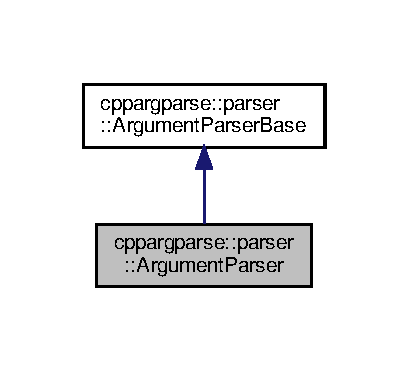
\includegraphics[width=196pt]{classcppargparse_1_1parser_1_1ArgumentParser__inherit__graph}
\end{center}
\end{figure}


Collaboration diagram for cppargparse\+:\+:parser\+:\+:Argument\+Parser\+:
\nopagebreak
\begin{figure}[H]
\begin{center}
\leavevmode
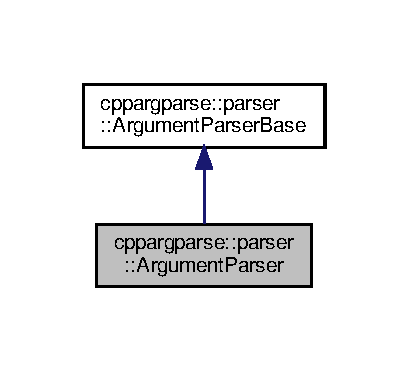
\includegraphics[width=196pt]{classcppargparse_1_1parser_1_1ArgumentParser__coll__graph}
\end{center}
\end{figure}
\subsection*{Public Member Functions}
\begin{DoxyCompactItemize}
\item 
\hyperlink{classcppargparse_1_1parser_1_1ArgumentParser_a704fa488168e08c7ae727445c5fa710a}{Argument\+Parser} (int argc, char $\ast$argv\mbox{[}$\,$\mbox{]}, const std\+::string \&application\+\_\+description)
\begin{DoxyCompactList}\small\item\em c\textquotesingle{}tor \end{DoxyCompactList}\item 
{\footnotesize template$<$typename T $>$ }\\const T \hyperlink{classcppargparse_1_1parser_1_1ArgumentParser_a3e8d3ae0eece40b7e62ae6faae5107ed}{get\+\_\+option} (const std\+::string \&id)
\begin{DoxyCompactList}\small\item\em Return an argument value. \end{DoxyCompactList}\item 
{\footnotesize template$<$typename T $>$ }\\const T \hyperlink{classcppargparse_1_1parser_1_1ArgumentParser_a6e13da383b8fdac04a35767abe0f5c32}{get\+\_\+option} (const std\+::string \&id, const T \&default\+\_\+value)
\begin{DoxyCompactList}\small\item\em Return an argument value. \end{DoxyCompactList}\item 
void \hyperlink{classcppargparse_1_1parser_1_1ArgumentParser_aa9abf9b86b7310784d04085cff2a4d3c}{add\+\_\+flag\+\_\+with\+\_\+callback} (const std\+::string \&id, const std\+::function$<$ void(const \hyperlink{classcppargparse_1_1parser_1_1ArgumentParser}{Argument\+Parser} \&)$>$ \&callback)
\begin{DoxyCompactList}\small\item\em Add a flag argument and call a callback when it has been passed to the command line. \end{DoxyCompactList}\item 
void \hyperlink{classcppargparse_1_1parser_1_1ArgumentParser_ac117877909d58e4a18d6a5094c2c6877}{add\+\_\+flag\+\_\+with\+\_\+callback} (const std\+::string \&id, const std\+::string \&id\+\_\+alt, const std\+::function$<$ void(const \hyperlink{classcppargparse_1_1parser_1_1ArgumentParser}{Argument\+Parser} \&)$>$ \&callback)
\begin{DoxyCompactList}\small\item\em Add a flag argument and call a callback when it has been passed to the command line. \end{DoxyCompactList}\item 
void \hyperlink{classcppargparse_1_1parser_1_1ArgumentParser_a6c466f78b14f49750ef608e3a5977b74}{add\+\_\+flag\+\_\+with\+\_\+callback} (const std\+::string \&id, const std\+::string \&id\+\_\+alt, const std\+::string \&description, const std\+::function$<$ void(const \hyperlink{classcppargparse_1_1parser_1_1ArgumentParser}{Argument\+Parser} \&)$>$ \&callback)
\begin{DoxyCompactList}\small\item\em Add a flag argument and call a callback when it has been passed to the command line. \end{DoxyCompactList}\item 
void \hyperlink{classcppargparse_1_1parser_1_1ArgumentParser_a5763e301e54e619c96d9364f75b1d4c9}{add\+\_\+help\+\_\+with\+\_\+callback} (const std\+::function$<$ void(const \hyperlink{classcppargparse_1_1parser_1_1ArgumentParser}{Argument\+Parser} \&)$>$ \&callback)
\begin{DoxyCompactList}\small\item\em Add the default help argument (-\/h, --help) and call a callback when it has been passed to the command line. \end{DoxyCompactList}\item 
{\footnotesize template$<$typename T $>$ }\\void \hyperlink{classcppargparse_1_1parser_1_1ArgumentParser_aad667a38fb847cd48b15f66cb99c1818}{add\+\_\+arg\+\_\+with\+\_\+callback} (const std\+::string \&id, const std\+::function$<$ void(const \hyperlink{classcppargparse_1_1parser_1_1ArgumentParser}{Argument\+Parser} \&, const T \&)$>$ \&callback)
\begin{DoxyCompactList}\small\item\em Add an argument and call a callback with its value when it has been passed to the command line. \end{DoxyCompactList}\item 
{\footnotesize template$<$typename T $>$ }\\void \hyperlink{classcppargparse_1_1parser_1_1ArgumentParser_a303a12481a661f3d38c66718d6e593a7}{add\+\_\+arg\+\_\+with\+\_\+callback} (const std\+::string \&id, const std\+::string \&id\+\_\+alt, const std\+::function$<$ void(const \hyperlink{classcppargparse_1_1parser_1_1ArgumentParser}{Argument\+Parser} \&, const T \&)$>$ \&callback)
\begin{DoxyCompactList}\small\item\em Add an argument and call a callback with its value when it has been passed to the command line. \end{DoxyCompactList}\item 
{\footnotesize template$<$typename T $>$ }\\void \hyperlink{classcppargparse_1_1parser_1_1ArgumentParser_aace5e7d0b1dd1831bc06ae7d3c3f2725}{add\+\_\+arg\+\_\+with\+\_\+callback} (const std\+::string \&id, const std\+::string \&id\+\_\+alt, const std\+::string \&description, const std\+::function$<$ void(const \hyperlink{classcppargparse_1_1parser_1_1ArgumentParser}{Argument\+Parser} \&, const T \&)$>$ \&callback)
\begin{DoxyCompactList}\small\item\em Add an argument and call a callback with its value when it has been passed to the command line. \end{DoxyCompactList}\item 
{\footnotesize template$<$typename T $>$ }\\void \hyperlink{classcppargparse_1_1parser_1_1ArgumentParser_a63d7feb48b03e26cc64ccd22382685d4}{add\+\_\+arg\+\_\+with\+\_\+callback\+\_\+default} (const std\+::string \&id, const T \&default\+\_\+value, const std\+::function$<$ void(const \hyperlink{classcppargparse_1_1parser_1_1ArgumentParser}{Argument\+Parser} \&, const T \&)$>$ \&callback)
\begin{DoxyCompactList}\small\item\em Add an argument and call a callback with its (default) value. \end{DoxyCompactList}\item 
{\footnotesize template$<$typename T $>$ }\\void \hyperlink{classcppargparse_1_1parser_1_1ArgumentParser_a8bc57f2778cc9ba82dfd0f255376ab4a}{add\+\_\+arg\+\_\+with\+\_\+callback\+\_\+default} (const std\+::string \&id, const std\+::string \&id\+\_\+alt, const T \&default\+\_\+value, const std\+::function$<$ void(const \hyperlink{classcppargparse_1_1parser_1_1ArgumentParser}{Argument\+Parser} \&, const T \&)$>$ \&callback)
\begin{DoxyCompactList}\small\item\em Add an argument and call a callback with its (default) value. \end{DoxyCompactList}\item 
{\footnotesize template$<$typename T $>$ }\\void \hyperlink{classcppargparse_1_1parser_1_1ArgumentParser_a4693605cbe40d87c0a23546a5e61fa97}{add\+\_\+arg\+\_\+with\+\_\+callback\+\_\+default} (const std\+::string \&id, const std\+::string \&id\+\_\+alt, const std\+::string \&description, const T \&default\+\_\+value, const std\+::function$<$ void(const \hyperlink{classcppargparse_1_1parser_1_1ArgumentParser}{Argument\+Parser} \&, const T \&)$>$ \&callback)
\begin{DoxyCompactList}\small\item\em Add an argument and call a callback with its (default) value. \end{DoxyCompactList}\end{DoxyCompactItemize}
\subsection*{Additional Inherited Members}


\subsection{Detailed Description}
The argument parser class. 

Used as an interface between the argument value conversion operations and the outside world. 

\subsection{Constructor \& Destructor Documentation}
\mbox{\Hypertarget{classcppargparse_1_1parser_1_1ArgumentParser_a704fa488168e08c7ae727445c5fa710a}\label{classcppargparse_1_1parser_1_1ArgumentParser_a704fa488168e08c7ae727445c5fa710a}} 
\index{cppargparse\+::parser\+::\+Argument\+Parser@{cppargparse\+::parser\+::\+Argument\+Parser}!Argument\+Parser@{Argument\+Parser}}
\index{Argument\+Parser@{Argument\+Parser}!cppargparse\+::parser\+::\+Argument\+Parser@{cppargparse\+::parser\+::\+Argument\+Parser}}
\subsubsection{\texorpdfstring{Argument\+Parser()}{ArgumentParser()}}
{\footnotesize\ttfamily cppargparse\+::parser\+::\+Argument\+Parser\+::\+Argument\+Parser (\begin{DoxyParamCaption}\item[{int}]{argc,  }\item[{char $\ast$}]{argv\mbox{[}$\,$\mbox{]},  }\item[{const std\+::string \&}]{application\+\_\+description }\end{DoxyParamCaption})\hspace{0.3cm}{\ttfamily [inline]}, {\ttfamily [explicit]}}



c\textquotesingle{}tor 


\begin{DoxyParams}{Parameters}
{\em argc} & The command line argument count. \\
\hline
{\em argv} & The command line argument array. \\
\hline
{\em application\+\_\+description} & The application description. \\
\hline
\end{DoxyParams}


\subsection{Member Function Documentation}
\mbox{\Hypertarget{classcppargparse_1_1parser_1_1ArgumentParser_aad667a38fb847cd48b15f66cb99c1818}\label{classcppargparse_1_1parser_1_1ArgumentParser_aad667a38fb847cd48b15f66cb99c1818}} 
\index{cppargparse\+::parser\+::\+Argument\+Parser@{cppargparse\+::parser\+::\+Argument\+Parser}!add\+\_\+arg\+\_\+with\+\_\+callback@{add\+\_\+arg\+\_\+with\+\_\+callback}}
\index{add\+\_\+arg\+\_\+with\+\_\+callback@{add\+\_\+arg\+\_\+with\+\_\+callback}!cppargparse\+::parser\+::\+Argument\+Parser@{cppargparse\+::parser\+::\+Argument\+Parser}}
\subsubsection{\texorpdfstring{add\+\_\+arg\+\_\+with\+\_\+callback()}{add\_arg\_with\_callback()}\hspace{0.1cm}{\footnotesize\ttfamily [1/3]}}
{\footnotesize\ttfamily template$<$typename T $>$ \\
void cppargparse\+::parser\+::\+Argument\+Parser\+::add\+\_\+arg\+\_\+with\+\_\+callback (\begin{DoxyParamCaption}\item[{const std\+::string \&}]{id,  }\item[{const std\+::function$<$ void(const \hyperlink{classcppargparse_1_1parser_1_1ArgumentParser}{Argument\+Parser} \&, const T \&)$>$ \&}]{callback }\end{DoxyParamCaption})\hspace{0.3cm}{\ttfamily [inline]}}



Add an argument and call a callback with its value when it has been passed to the command line. 


\begin{DoxyTemplParams}{Template Parameters}
{\em T} & The argument value type.\\
\hline
\end{DoxyTemplParams}

\begin{DoxyParams}{Parameters}
{\em id} & The argument ID. \\
\hline
{\em callback} & The callback to call with the argument\textquotesingle{}s value when the argument has been passed to the command line.\\
\hline
\end{DoxyParams}

\begin{DoxyExceptions}{Exceptions}
{\em \#errors\+::\+Command\+Line\+Argument\+Error} & if the arg wasn\textquotesingle{}t found in the command line. \\
\hline
{\em \#errors\+::\+Command\+Line\+Option\+Error} & if no value has been found for the argument. \\
\hline
\end{DoxyExceptions}
\mbox{\Hypertarget{classcppargparse_1_1parser_1_1ArgumentParser_a303a12481a661f3d38c66718d6e593a7}\label{classcppargparse_1_1parser_1_1ArgumentParser_a303a12481a661f3d38c66718d6e593a7}} 
\index{cppargparse\+::parser\+::\+Argument\+Parser@{cppargparse\+::parser\+::\+Argument\+Parser}!add\+\_\+arg\+\_\+with\+\_\+callback@{add\+\_\+arg\+\_\+with\+\_\+callback}}
\index{add\+\_\+arg\+\_\+with\+\_\+callback@{add\+\_\+arg\+\_\+with\+\_\+callback}!cppargparse\+::parser\+::\+Argument\+Parser@{cppargparse\+::parser\+::\+Argument\+Parser}}
\subsubsection{\texorpdfstring{add\+\_\+arg\+\_\+with\+\_\+callback()}{add\_arg\_with\_callback()}\hspace{0.1cm}{\footnotesize\ttfamily [2/3]}}
{\footnotesize\ttfamily template$<$typename T $>$ \\
void cppargparse\+::parser\+::\+Argument\+Parser\+::add\+\_\+arg\+\_\+with\+\_\+callback (\begin{DoxyParamCaption}\item[{const std\+::string \&}]{id,  }\item[{const std\+::string \&}]{id\+\_\+alt,  }\item[{const std\+::function$<$ void(const \hyperlink{classcppargparse_1_1parser_1_1ArgumentParser}{Argument\+Parser} \&, const T \&)$>$ \&}]{callback }\end{DoxyParamCaption})\hspace{0.3cm}{\ttfamily [inline]}}



Add an argument and call a callback with its value when it has been passed to the command line. 


\begin{DoxyTemplParams}{Template Parameters}
{\em T} & The argument value type.\\
\hline
\end{DoxyTemplParams}

\begin{DoxyParams}{Parameters}
{\em id} & The argument ID. \\
\hline
{\em id\+\_\+alt} & The argument alternative ID. \\
\hline
{\em callback} & The callback to call with the argument\textquotesingle{}s value when the argument has been passed to the command line.\\
\hline
\end{DoxyParams}

\begin{DoxyExceptions}{Exceptions}
{\em \#errors\+::\+Command\+Line\+Argument\+Error} & if the arg wasn\textquotesingle{}t found in the command line. \\
\hline
{\em \#errors\+::\+Command\+Line\+Option\+Error} & if no value has been found for the argument. \\
\hline
\end{DoxyExceptions}
\mbox{\Hypertarget{classcppargparse_1_1parser_1_1ArgumentParser_aace5e7d0b1dd1831bc06ae7d3c3f2725}\label{classcppargparse_1_1parser_1_1ArgumentParser_aace5e7d0b1dd1831bc06ae7d3c3f2725}} 
\index{cppargparse\+::parser\+::\+Argument\+Parser@{cppargparse\+::parser\+::\+Argument\+Parser}!add\+\_\+arg\+\_\+with\+\_\+callback@{add\+\_\+arg\+\_\+with\+\_\+callback}}
\index{add\+\_\+arg\+\_\+with\+\_\+callback@{add\+\_\+arg\+\_\+with\+\_\+callback}!cppargparse\+::parser\+::\+Argument\+Parser@{cppargparse\+::parser\+::\+Argument\+Parser}}
\subsubsection{\texorpdfstring{add\+\_\+arg\+\_\+with\+\_\+callback()}{add\_arg\_with\_callback()}\hspace{0.1cm}{\footnotesize\ttfamily [3/3]}}
{\footnotesize\ttfamily template$<$typename T $>$ \\
void cppargparse\+::parser\+::\+Argument\+Parser\+::add\+\_\+arg\+\_\+with\+\_\+callback (\begin{DoxyParamCaption}\item[{const std\+::string \&}]{id,  }\item[{const std\+::string \&}]{id\+\_\+alt,  }\item[{const std\+::string \&}]{description,  }\item[{const std\+::function$<$ void(const \hyperlink{classcppargparse_1_1parser_1_1ArgumentParser}{Argument\+Parser} \&, const T \&)$>$ \&}]{callback }\end{DoxyParamCaption})\hspace{0.3cm}{\ttfamily [inline]}}



Add an argument and call a callback with its value when it has been passed to the command line. 


\begin{DoxyTemplParams}{Template Parameters}
{\em T} & The argument value type.\\
\hline
\end{DoxyTemplParams}

\begin{DoxyParams}{Parameters}
{\em id} & The argument ID. \\
\hline
{\em id\+\_\+alt} & The argument alternative ID. \\
\hline
{\em description} & The argument description. \\
\hline
{\em callback} & The callback to call with the argument\textquotesingle{}s value when the argument has been passed to the command line.\\
\hline
\end{DoxyParams}

\begin{DoxyExceptions}{Exceptions}
{\em \#errors\+::\+Command\+Line\+Argument\+Error} & if the arg wasn\textquotesingle{}t found in the command line. \\
\hline
{\em \#errors\+::\+Command\+Line\+Option\+Error} & if no value has been found for the argument. \\
\hline
\end{DoxyExceptions}
\mbox{\Hypertarget{classcppargparse_1_1parser_1_1ArgumentParser_a63d7feb48b03e26cc64ccd22382685d4}\label{classcppargparse_1_1parser_1_1ArgumentParser_a63d7feb48b03e26cc64ccd22382685d4}} 
\index{cppargparse\+::parser\+::\+Argument\+Parser@{cppargparse\+::parser\+::\+Argument\+Parser}!add\+\_\+arg\+\_\+with\+\_\+callback\+\_\+default@{add\+\_\+arg\+\_\+with\+\_\+callback\+\_\+default}}
\index{add\+\_\+arg\+\_\+with\+\_\+callback\+\_\+default@{add\+\_\+arg\+\_\+with\+\_\+callback\+\_\+default}!cppargparse\+::parser\+::\+Argument\+Parser@{cppargparse\+::parser\+::\+Argument\+Parser}}
\subsubsection{\texorpdfstring{add\+\_\+arg\+\_\+with\+\_\+callback\+\_\+default()}{add\_arg\_with\_callback\_default()}\hspace{0.1cm}{\footnotesize\ttfamily [1/3]}}
{\footnotesize\ttfamily template$<$typename T $>$ \\
void cppargparse\+::parser\+::\+Argument\+Parser\+::add\+\_\+arg\+\_\+with\+\_\+callback\+\_\+default (\begin{DoxyParamCaption}\item[{const std\+::string \&}]{id,  }\item[{const T \&}]{default\+\_\+value,  }\item[{const std\+::function$<$ void(const \hyperlink{classcppargparse_1_1parser_1_1ArgumentParser}{Argument\+Parser} \&, const T \&)$>$ \&}]{callback }\end{DoxyParamCaption})\hspace{0.3cm}{\ttfamily [inline]}}



Add an argument and call a callback with its (default) value. 


\begin{DoxyTemplParams}{Template Parameters}
{\em T} & The argument value type.\\
\hline
\end{DoxyTemplParams}

\begin{DoxyParams}{Parameters}
{\em id} & The argument ID. \\
\hline
{\em default\+\_\+value} & The default value. \\
\hline
{\em callback} & The callback to call with the argument\textquotesingle{}s (default) value. \\
\hline
\end{DoxyParams}
\mbox{\Hypertarget{classcppargparse_1_1parser_1_1ArgumentParser_a8bc57f2778cc9ba82dfd0f255376ab4a}\label{classcppargparse_1_1parser_1_1ArgumentParser_a8bc57f2778cc9ba82dfd0f255376ab4a}} 
\index{cppargparse\+::parser\+::\+Argument\+Parser@{cppargparse\+::parser\+::\+Argument\+Parser}!add\+\_\+arg\+\_\+with\+\_\+callback\+\_\+default@{add\+\_\+arg\+\_\+with\+\_\+callback\+\_\+default}}
\index{add\+\_\+arg\+\_\+with\+\_\+callback\+\_\+default@{add\+\_\+arg\+\_\+with\+\_\+callback\+\_\+default}!cppargparse\+::parser\+::\+Argument\+Parser@{cppargparse\+::parser\+::\+Argument\+Parser}}
\subsubsection{\texorpdfstring{add\+\_\+arg\+\_\+with\+\_\+callback\+\_\+default()}{add\_arg\_with\_callback\_default()}\hspace{0.1cm}{\footnotesize\ttfamily [2/3]}}
{\footnotesize\ttfamily template$<$typename T $>$ \\
void cppargparse\+::parser\+::\+Argument\+Parser\+::add\+\_\+arg\+\_\+with\+\_\+callback\+\_\+default (\begin{DoxyParamCaption}\item[{const std\+::string \&}]{id,  }\item[{const std\+::string \&}]{id\+\_\+alt,  }\item[{const T \&}]{default\+\_\+value,  }\item[{const std\+::function$<$ void(const \hyperlink{classcppargparse_1_1parser_1_1ArgumentParser}{Argument\+Parser} \&, const T \&)$>$ \&}]{callback }\end{DoxyParamCaption})\hspace{0.3cm}{\ttfamily [inline]}}



Add an argument and call a callback with its (default) value. 


\begin{DoxyTemplParams}{Template Parameters}
{\em T} & The argument value type.\\
\hline
\end{DoxyTemplParams}

\begin{DoxyParams}{Parameters}
{\em id} & The argument ID. \\
\hline
{\em id\+\_\+alt} & The argument alternative ID. \\
\hline
{\em default\+\_\+value} & The default value. \\
\hline
{\em callback} & The callback to call with the argument\textquotesingle{}s (default) value. \\
\hline
\end{DoxyParams}
\mbox{\Hypertarget{classcppargparse_1_1parser_1_1ArgumentParser_a4693605cbe40d87c0a23546a5e61fa97}\label{classcppargparse_1_1parser_1_1ArgumentParser_a4693605cbe40d87c0a23546a5e61fa97}} 
\index{cppargparse\+::parser\+::\+Argument\+Parser@{cppargparse\+::parser\+::\+Argument\+Parser}!add\+\_\+arg\+\_\+with\+\_\+callback\+\_\+default@{add\+\_\+arg\+\_\+with\+\_\+callback\+\_\+default}}
\index{add\+\_\+arg\+\_\+with\+\_\+callback\+\_\+default@{add\+\_\+arg\+\_\+with\+\_\+callback\+\_\+default}!cppargparse\+::parser\+::\+Argument\+Parser@{cppargparse\+::parser\+::\+Argument\+Parser}}
\subsubsection{\texorpdfstring{add\+\_\+arg\+\_\+with\+\_\+callback\+\_\+default()}{add\_arg\_with\_callback\_default()}\hspace{0.1cm}{\footnotesize\ttfamily [3/3]}}
{\footnotesize\ttfamily template$<$typename T $>$ \\
void cppargparse\+::parser\+::\+Argument\+Parser\+::add\+\_\+arg\+\_\+with\+\_\+callback\+\_\+default (\begin{DoxyParamCaption}\item[{const std\+::string \&}]{id,  }\item[{const std\+::string \&}]{id\+\_\+alt,  }\item[{const std\+::string \&}]{description,  }\item[{const T \&}]{default\+\_\+value,  }\item[{const std\+::function$<$ void(const \hyperlink{classcppargparse_1_1parser_1_1ArgumentParser}{Argument\+Parser} \&, const T \&)$>$ \&}]{callback }\end{DoxyParamCaption})\hspace{0.3cm}{\ttfamily [inline]}}



Add an argument and call a callback with its (default) value. 


\begin{DoxyTemplParams}{Template Parameters}
{\em T} & The argument value type.\\
\hline
\end{DoxyTemplParams}

\begin{DoxyParams}{Parameters}
{\em id} & The argument ID. \\
\hline
{\em id\+\_\+alt} & The argument alternative ID. \\
\hline
{\em description} & The argument description. \\
\hline
{\em default\+\_\+value} & The default value. \\
\hline
{\em callback} & The callback to call with the argument\textquotesingle{}s (default) value. \\
\hline
\end{DoxyParams}
\mbox{\Hypertarget{classcppargparse_1_1parser_1_1ArgumentParser_aa9abf9b86b7310784d04085cff2a4d3c}\label{classcppargparse_1_1parser_1_1ArgumentParser_aa9abf9b86b7310784d04085cff2a4d3c}} 
\index{cppargparse\+::parser\+::\+Argument\+Parser@{cppargparse\+::parser\+::\+Argument\+Parser}!add\+\_\+flag\+\_\+with\+\_\+callback@{add\+\_\+flag\+\_\+with\+\_\+callback}}
\index{add\+\_\+flag\+\_\+with\+\_\+callback@{add\+\_\+flag\+\_\+with\+\_\+callback}!cppargparse\+::parser\+::\+Argument\+Parser@{cppargparse\+::parser\+::\+Argument\+Parser}}
\subsubsection{\texorpdfstring{add\+\_\+flag\+\_\+with\+\_\+callback()}{add\_flag\_with\_callback()}\hspace{0.1cm}{\footnotesize\ttfamily [1/3]}}
{\footnotesize\ttfamily void cppargparse\+::parser\+::\+Argument\+Parser\+::add\+\_\+flag\+\_\+with\+\_\+callback (\begin{DoxyParamCaption}\item[{const std\+::string \&}]{id,  }\item[{const std\+::function$<$ void(const \hyperlink{classcppargparse_1_1parser_1_1ArgumentParser}{Argument\+Parser} \&)$>$ \&}]{callback }\end{DoxyParamCaption})\hspace{0.3cm}{\ttfamily [inline]}}



Add a flag argument and call a callback when it has been passed to the command line. 


\begin{DoxyParams}{Parameters}
{\em id} & The argument ID. \\
\hline
{\em callback} & The callback to call when the flag has been passed to the command line. \\
\hline
\end{DoxyParams}
\mbox{\Hypertarget{classcppargparse_1_1parser_1_1ArgumentParser_ac117877909d58e4a18d6a5094c2c6877}\label{classcppargparse_1_1parser_1_1ArgumentParser_ac117877909d58e4a18d6a5094c2c6877}} 
\index{cppargparse\+::parser\+::\+Argument\+Parser@{cppargparse\+::parser\+::\+Argument\+Parser}!add\+\_\+flag\+\_\+with\+\_\+callback@{add\+\_\+flag\+\_\+with\+\_\+callback}}
\index{add\+\_\+flag\+\_\+with\+\_\+callback@{add\+\_\+flag\+\_\+with\+\_\+callback}!cppargparse\+::parser\+::\+Argument\+Parser@{cppargparse\+::parser\+::\+Argument\+Parser}}
\subsubsection{\texorpdfstring{add\+\_\+flag\+\_\+with\+\_\+callback()}{add\_flag\_with\_callback()}\hspace{0.1cm}{\footnotesize\ttfamily [2/3]}}
{\footnotesize\ttfamily void cppargparse\+::parser\+::\+Argument\+Parser\+::add\+\_\+flag\+\_\+with\+\_\+callback (\begin{DoxyParamCaption}\item[{const std\+::string \&}]{id,  }\item[{const std\+::string \&}]{id\+\_\+alt,  }\item[{const std\+::function$<$ void(const \hyperlink{classcppargparse_1_1parser_1_1ArgumentParser}{Argument\+Parser} \&)$>$ \&}]{callback }\end{DoxyParamCaption})\hspace{0.3cm}{\ttfamily [inline]}}



Add a flag argument and call a callback when it has been passed to the command line. 


\begin{DoxyParams}{Parameters}
{\em id} & The argument ID. \\
\hline
{\em id\+\_\+alt} & The argument alternative ID. \\
\hline
{\em callback} & The callback to call when the flag has been passed to the command line. \\
\hline
\end{DoxyParams}
\mbox{\Hypertarget{classcppargparse_1_1parser_1_1ArgumentParser_a6c466f78b14f49750ef608e3a5977b74}\label{classcppargparse_1_1parser_1_1ArgumentParser_a6c466f78b14f49750ef608e3a5977b74}} 
\index{cppargparse\+::parser\+::\+Argument\+Parser@{cppargparse\+::parser\+::\+Argument\+Parser}!add\+\_\+flag\+\_\+with\+\_\+callback@{add\+\_\+flag\+\_\+with\+\_\+callback}}
\index{add\+\_\+flag\+\_\+with\+\_\+callback@{add\+\_\+flag\+\_\+with\+\_\+callback}!cppargparse\+::parser\+::\+Argument\+Parser@{cppargparse\+::parser\+::\+Argument\+Parser}}
\subsubsection{\texorpdfstring{add\+\_\+flag\+\_\+with\+\_\+callback()}{add\_flag\_with\_callback()}\hspace{0.1cm}{\footnotesize\ttfamily [3/3]}}
{\footnotesize\ttfamily void cppargparse\+::parser\+::\+Argument\+Parser\+::add\+\_\+flag\+\_\+with\+\_\+callback (\begin{DoxyParamCaption}\item[{const std\+::string \&}]{id,  }\item[{const std\+::string \&}]{id\+\_\+alt,  }\item[{const std\+::string \&}]{description,  }\item[{const std\+::function$<$ void(const \hyperlink{classcppargparse_1_1parser_1_1ArgumentParser}{Argument\+Parser} \&)$>$ \&}]{callback }\end{DoxyParamCaption})\hspace{0.3cm}{\ttfamily [inline]}}



Add a flag argument and call a callback when it has been passed to the command line. 


\begin{DoxyParams}{Parameters}
{\em id} & The argument ID. \\
\hline
{\em id\+\_\+alt} & The argument alternative ID. \\
\hline
{\em description} & The argument description. \\
\hline
{\em callback} & The callback to call when the flag has been passed to the command line. \\
\hline
\end{DoxyParams}
\mbox{\Hypertarget{classcppargparse_1_1parser_1_1ArgumentParser_a5763e301e54e619c96d9364f75b1d4c9}\label{classcppargparse_1_1parser_1_1ArgumentParser_a5763e301e54e619c96d9364f75b1d4c9}} 
\index{cppargparse\+::parser\+::\+Argument\+Parser@{cppargparse\+::parser\+::\+Argument\+Parser}!add\+\_\+help\+\_\+with\+\_\+callback@{add\+\_\+help\+\_\+with\+\_\+callback}}
\index{add\+\_\+help\+\_\+with\+\_\+callback@{add\+\_\+help\+\_\+with\+\_\+callback}!cppargparse\+::parser\+::\+Argument\+Parser@{cppargparse\+::parser\+::\+Argument\+Parser}}
\subsubsection{\texorpdfstring{add\+\_\+help\+\_\+with\+\_\+callback()}{add\_help\_with\_callback()}}
{\footnotesize\ttfamily void cppargparse\+::parser\+::\+Argument\+Parser\+::add\+\_\+help\+\_\+with\+\_\+callback (\begin{DoxyParamCaption}\item[{const std\+::function$<$ void(const \hyperlink{classcppargparse_1_1parser_1_1ArgumentParser}{Argument\+Parser} \&)$>$ \&}]{callback }\end{DoxyParamCaption})\hspace{0.3cm}{\ttfamily [inline]}}



Add the default help argument (-\/h, --help) and call a callback when it has been passed to the command line. 


\begin{DoxyParams}{Parameters}
{\em callback} & The callback to call when the flag has been passed to the command line. \\
\hline
\end{DoxyParams}
\mbox{\Hypertarget{classcppargparse_1_1parser_1_1ArgumentParser_a3e8d3ae0eece40b7e62ae6faae5107ed}\label{classcppargparse_1_1parser_1_1ArgumentParser_a3e8d3ae0eece40b7e62ae6faae5107ed}} 
\index{cppargparse\+::parser\+::\+Argument\+Parser@{cppargparse\+::parser\+::\+Argument\+Parser}!get\+\_\+option@{get\+\_\+option}}
\index{get\+\_\+option@{get\+\_\+option}!cppargparse\+::parser\+::\+Argument\+Parser@{cppargparse\+::parser\+::\+Argument\+Parser}}
\subsubsection{\texorpdfstring{get\+\_\+option()}{get\_option()}\hspace{0.1cm}{\footnotesize\ttfamily [1/2]}}
{\footnotesize\ttfamily template$<$typename T $>$ \\
const T cppargparse\+::parser\+::\+Argument\+Parser\+::get\+\_\+option (\begin{DoxyParamCaption}\item[{const std\+::string \&}]{id }\end{DoxyParamCaption})\hspace{0.3cm}{\ttfamily [inline]}}



Return an argument value. 


\begin{DoxyTemplParams}{Template Parameters}
{\em T} & The argument type. \hyperlink{structcppargparse_1_1argument_a9b5feac6fe8cf18beb63d85c0840cd84}{argument\+::parse()} and \hyperlink{structcppargparse_1_1argument_a2051f71ef4ed0b9d299cc58bb494e42b}{argument\+::convert()} must be implemented for T.\\
\hline
\end{DoxyTemplParams}

\begin{DoxyParams}{Parameters}
{\em id} & The argument ID. Can also be the argument\textquotesingle{}s alternative ID.\\
\hline
\end{DoxyParams}
\begin{DoxyReturn}{Returns}
The argument value of type T. 
\end{DoxyReturn}

\begin{DoxyExceptions}{Exceptions}
{\em \hyperlink{classcppargparse_1_1errors_1_1CommandLineArgumentError}{cppargparse\+::errors\+::\+Command\+Line\+Argument\+Error}} & if the argument cannot be found. \\
\hline
\end{DoxyExceptions}
\mbox{\Hypertarget{classcppargparse_1_1parser_1_1ArgumentParser_a6e13da383b8fdac04a35767abe0f5c32}\label{classcppargparse_1_1parser_1_1ArgumentParser_a6e13da383b8fdac04a35767abe0f5c32}} 
\index{cppargparse\+::parser\+::\+Argument\+Parser@{cppargparse\+::parser\+::\+Argument\+Parser}!get\+\_\+option@{get\+\_\+option}}
\index{get\+\_\+option@{get\+\_\+option}!cppargparse\+::parser\+::\+Argument\+Parser@{cppargparse\+::parser\+::\+Argument\+Parser}}
\subsubsection{\texorpdfstring{get\+\_\+option()}{get\_option()}\hspace{0.1cm}{\footnotesize\ttfamily [2/2]}}
{\footnotesize\ttfamily template$<$typename T $>$ \\
const T cppargparse\+::parser\+::\+Argument\+Parser\+::get\+\_\+option (\begin{DoxyParamCaption}\item[{const std\+::string \&}]{id,  }\item[{const T \&}]{default\+\_\+value }\end{DoxyParamCaption})\hspace{0.3cm}{\ttfamily [inline]}}



Return an argument value. 


\begin{DoxyTemplParams}{Template Parameters}
{\em T} & The argument type. \hyperlink{structcppargparse_1_1argument_a9b5feac6fe8cf18beb63d85c0840cd84}{argument\+::parse()} and \hyperlink{structcppargparse_1_1argument_a2051f71ef4ed0b9d299cc58bb494e42b}{argument\+::convert()} must be implemented for T.\\
\hline
\end{DoxyTemplParams}

\begin{DoxyParams}{Parameters}
{\em id} & The argument string. Can also be the argument\textquotesingle{}s alternative ID. \\
\hline
{\em default\+\_\+value} & The default argument value of type T.\\
\hline
\end{DoxyParams}
\begin{DoxyReturn}{Returns}
The argument value of type T or the default value if the argument cannot be found. 
\end{DoxyReturn}

\begin{DoxyExceptions}{Exceptions}
{\em \hyperlink{classcppargparse_1_1errors_1_1CommandLineArgumentError}{cppargparse\+::errors\+::\+Command\+Line\+Argument\+Error}} & if the argument cannot be found \\
\hline
\end{DoxyExceptions}


The documentation for this class was generated from the following file\+:\begin{DoxyCompactItemize}
\item 
include/cppargparse/parser.\+h\end{DoxyCompactItemize}

\hypertarget{classcppargparse_1_1parser_1_1ArgumentParserBase}{}\section{cppargparse\+:\+:parser\+:\+:Argument\+Parser\+Base Class Reference}
\label{classcppargparse_1_1parser_1_1ArgumentParserBase}\index{cppargparse\+::parser\+::\+Argument\+Parser\+Base@{cppargparse\+::parser\+::\+Argument\+Parser\+Base}}


Base class for the argument parser.  




{\ttfamily \#include $<$parser.\+h$>$}



Inheritance diagram for cppargparse\+:\+:parser\+:\+:Argument\+Parser\+Base\+:\nopagebreak
\begin{figure}[H]
\begin{center}
\leavevmode
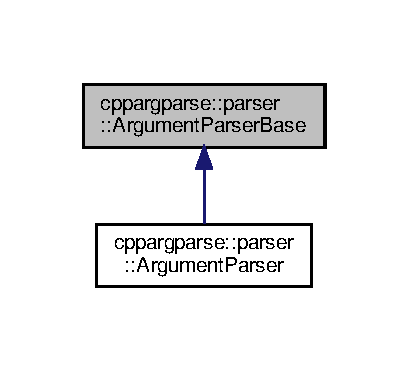
\includegraphics[width=196pt]{classcppargparse_1_1parser_1_1ArgumentParserBase__inherit__graph}
\end{center}
\end{figure}
\subsection*{Public Member Functions}
\begin{DoxyCompactItemize}
\item 
\hyperlink{classcppargparse_1_1parser_1_1ArgumentParserBase_a91c5c101e21966fb8c04c094b04b8ba3}{Argument\+Parser\+Base} (int argc, char $\ast$argv\mbox{[}$\,$\mbox{]}, const std\+::string \&application\+\_\+description)
\begin{DoxyCompactList}\small\item\em c\textquotesingle{}tor \end{DoxyCompactList}\item 
\hyperlink{classcppargparse_1_1parser_1_1ArgumentParserBase_a160867551ad33fceb69f9e920e3e4c23}{$\sim$\+Argument\+Parser\+Base} ()
\begin{DoxyCompactList}\small\item\em d\textquotesingle{}tor \end{DoxyCompactList}\item 
void \hyperlink{classcppargparse_1_1parser_1_1ArgumentParserBase_a2e1cc11e023a40d31881832331faa4b3}{add\+\_\+arg} (const \hyperlink{structcppargparse_1_1types_1_1CommandLineArgument__t}{types\+::\+Command\+Line\+Argument\+\_\+t} \&cmdarg)
\begin{DoxyCompactList}\small\item\em Add an argument to the command line arguments list. \end{DoxyCompactList}\item 
const \hyperlink{structcppargparse_1_1types_1_1CommandLineArgument__t}{types\+::\+Command\+Line\+Argument\+\_\+t} \hyperlink{classcppargparse_1_1parser_1_1ArgumentParserBase_a96ada5337bcd8898f630f83c9ecac523}{add\+\_\+arg} (const std\+::string \&id)
\begin{DoxyCompactList}\small\item\em Add an argument to the command line arguments list. \end{DoxyCompactList}\item 
const \hyperlink{structcppargparse_1_1types_1_1CommandLineArgument__t}{types\+::\+Command\+Line\+Argument\+\_\+t} \hyperlink{classcppargparse_1_1parser_1_1ArgumentParserBase_a4a0c6460abc3808c017de576052fa131}{add\+\_\+arg} (const std\+::string \&id, const std\+::string \&id\+\_\+alt)
\begin{DoxyCompactList}\small\item\em Add an argument to the command line arguments list. \end{DoxyCompactList}\item 
const \hyperlink{structcppargparse_1_1types_1_1CommandLineArgument__t}{types\+::\+Command\+Line\+Argument\+\_\+t} \hyperlink{classcppargparse_1_1parser_1_1ArgumentParserBase_ad1bb9bf2be4793b3442679fa2090bc2d}{add\+\_\+arg} (const std\+::string \&id, const std\+::string \&id\+\_\+alt, const std\+::string \&description)
\begin{DoxyCompactList}\small\item\em Add an argument to the command line arguments list. \end{DoxyCompactList}\item 
\mbox{\Hypertarget{classcppargparse_1_1parser_1_1ArgumentParserBase_aaa2d68da1d224500fa290040de72ff01}\label{classcppargparse_1_1parser_1_1ArgumentParserBase_aaa2d68da1d224500fa290040de72ff01}} 
const \hyperlink{structcppargparse_1_1types_1_1CommandLineArgument__t}{types\+::\+Command\+Line\+Argument\+\_\+t} \hyperlink{classcppargparse_1_1parser_1_1ArgumentParserBase_aaa2d68da1d224500fa290040de72ff01}{add\+\_\+help} ()
\begin{DoxyCompactList}\small\item\em Add default help argument\+: -\/h, --help. \end{DoxyCompactList}\item 
bool \hyperlink{classcppargparse_1_1parser_1_1ArgumentParserBase_aa95fba161ea60c65972e76025419b8d9}{get\+\_\+flag} (const \hyperlink{structcppargparse_1_1types_1_1CommandLineArgument__t}{types\+::\+Command\+Line\+Argument\+\_\+t} \&cmdarg)
\begin{DoxyCompactList}\small\item\em Return whether the command line contains an argument string. \end{DoxyCompactList}\item 
{\footnotesize template$<$typename T $>$ }\\const T \hyperlink{classcppargparse_1_1parser_1_1ArgumentParserBase_ae26532c710a553810a784d2243572e34}{get\+\_\+option} (const \hyperlink{structcppargparse_1_1types_1_1CommandLineArgument__t}{types\+::\+Command\+Line\+Argument\+\_\+t} \&)
\begin{DoxyCompactList}\small\item\em Stub method for returning an argument value. \end{DoxyCompactList}\item 
{\footnotesize template$<$typename T $>$ }\\const T \hyperlink{classcppargparse_1_1parser_1_1ArgumentParserBase_ae5f8dfec70ef927bc315e39046dcf63e}{get\+\_\+option} (const \hyperlink{structcppargparse_1_1types_1_1CommandLineArgument__t}{types\+::\+Command\+Line\+Argument\+\_\+t} \&, const T \&default\+\_\+value)
\begin{DoxyCompactList}\small\item\em Stub method for returning an argument value. \end{DoxyCompactList}\item 
const std\+::string \hyperlink{classcppargparse_1_1parser_1_1ArgumentParserBase_af99c2847a2cd19b1444dcb9ab2fb8103}{usage} () const
\begin{DoxyCompactList}\small\item\em Generate and return the usage string. \end{DoxyCompactList}\end{DoxyCompactItemize}
\subsection*{Protected Attributes}
\begin{DoxyCompactItemize}
\item 
\mbox{\Hypertarget{classcppargparse_1_1parser_1_1ArgumentParserBase_ab61aac285e831ef24598191816bed84d}\label{classcppargparse_1_1parser_1_1ArgumentParserBase_ab61aac285e831ef24598191816bed84d}} 
types\+::\+Command\+Line\+\_\+t \hyperlink{classcppargparse_1_1parser_1_1ArgumentParserBase_ab61aac285e831ef24598191816bed84d}{m\+\_\+cmd}
\begin{DoxyCompactList}\small\item\em The command line. \end{DoxyCompactList}\item 
\mbox{\Hypertarget{classcppargparse_1_1parser_1_1ArgumentParserBase_ac6fd162f8dfee569bb281ae5ef576d38}\label{classcppargparse_1_1parser_1_1ArgumentParserBase_ac6fd162f8dfee569bb281ae5ef576d38}} 
types\+::\+Command\+Line\+Arguments\+\_\+t \hyperlink{classcppargparse_1_1parser_1_1ArgumentParserBase_ac6fd162f8dfee569bb281ae5ef576d38}{m\+\_\+cmdargs}
\begin{DoxyCompactList}\small\item\em The command line arguments. \end{DoxyCompactList}\end{DoxyCompactItemize}


\subsection{Detailed Description}
Base class for the argument parser. 

\subsection{Constructor \& Destructor Documentation}
\mbox{\Hypertarget{classcppargparse_1_1parser_1_1ArgumentParserBase_a91c5c101e21966fb8c04c094b04b8ba3}\label{classcppargparse_1_1parser_1_1ArgumentParserBase_a91c5c101e21966fb8c04c094b04b8ba3}} 
\index{cppargparse\+::parser\+::\+Argument\+Parser\+Base@{cppargparse\+::parser\+::\+Argument\+Parser\+Base}!Argument\+Parser\+Base@{Argument\+Parser\+Base}}
\index{Argument\+Parser\+Base@{Argument\+Parser\+Base}!cppargparse\+::parser\+::\+Argument\+Parser\+Base@{cppargparse\+::parser\+::\+Argument\+Parser\+Base}}
\subsubsection{\texorpdfstring{Argument\+Parser\+Base()}{ArgumentParserBase()}}
{\footnotesize\ttfamily cppargparse\+::parser\+::\+Argument\+Parser\+Base\+::\+Argument\+Parser\+Base (\begin{DoxyParamCaption}\item[{int}]{argc,  }\item[{char $\ast$}]{argv\mbox{[}$\,$\mbox{]},  }\item[{const std\+::string \&}]{application\+\_\+description }\end{DoxyParamCaption})\hspace{0.3cm}{\ttfamily [inline]}, {\ttfamily [explicit]}}



c\textquotesingle{}tor 


\begin{DoxyParams}{Parameters}
{\em argc} & The command line argument count. \\
\hline
{\em argv} & The command line argument array. \\
\hline
{\em application\+\_\+description} & The application description. \\
\hline
\end{DoxyParams}
\mbox{\Hypertarget{classcppargparse_1_1parser_1_1ArgumentParserBase_a160867551ad33fceb69f9e920e3e4c23}\label{classcppargparse_1_1parser_1_1ArgumentParserBase_a160867551ad33fceb69f9e920e3e4c23}} 
\index{cppargparse\+::parser\+::\+Argument\+Parser\+Base@{cppargparse\+::parser\+::\+Argument\+Parser\+Base}!````~Argument\+Parser\+Base@{$\sim$\+Argument\+Parser\+Base}}
\index{````~Argument\+Parser\+Base@{$\sim$\+Argument\+Parser\+Base}!cppargparse\+::parser\+::\+Argument\+Parser\+Base@{cppargparse\+::parser\+::\+Argument\+Parser\+Base}}
\subsubsection{\texorpdfstring{$\sim$\+Argument\+Parser\+Base()}{~ArgumentParserBase()}}
{\footnotesize\ttfamily cppargparse\+::parser\+::\+Argument\+Parser\+Base\+::$\sim$\+Argument\+Parser\+Base (\begin{DoxyParamCaption}{ }\end{DoxyParamCaption})\hspace{0.3cm}{\ttfamily [inline]}}



d\textquotesingle{}tor 

Clean up storage for the command line and the command line argument map. 

\subsection{Member Function Documentation}
\mbox{\Hypertarget{classcppargparse_1_1parser_1_1ArgumentParserBase_a2e1cc11e023a40d31881832331faa4b3}\label{classcppargparse_1_1parser_1_1ArgumentParserBase_a2e1cc11e023a40d31881832331faa4b3}} 
\index{cppargparse\+::parser\+::\+Argument\+Parser\+Base@{cppargparse\+::parser\+::\+Argument\+Parser\+Base}!add\+\_\+arg@{add\+\_\+arg}}
\index{add\+\_\+arg@{add\+\_\+arg}!cppargparse\+::parser\+::\+Argument\+Parser\+Base@{cppargparse\+::parser\+::\+Argument\+Parser\+Base}}
\subsubsection{\texorpdfstring{add\+\_\+arg()}{add\_arg()}\hspace{0.1cm}{\footnotesize\ttfamily [1/4]}}
{\footnotesize\ttfamily void cppargparse\+::parser\+::\+Argument\+Parser\+Base\+::add\+\_\+arg (\begin{DoxyParamCaption}\item[{const \hyperlink{structcppargparse_1_1types_1_1CommandLineArgument__t}{types\+::\+Command\+Line\+Argument\+\_\+t} \&}]{cmdarg }\end{DoxyParamCaption})\hspace{0.3cm}{\ttfamily [inline]}}



Add an argument to the command line arguments list. 


\begin{DoxyParams}{Parameters}
{\em cmdarg} & The command line argument struct object. \\
\hline
\end{DoxyParams}
\mbox{\Hypertarget{classcppargparse_1_1parser_1_1ArgumentParserBase_a96ada5337bcd8898f630f83c9ecac523}\label{classcppargparse_1_1parser_1_1ArgumentParserBase_a96ada5337bcd8898f630f83c9ecac523}} 
\index{cppargparse\+::parser\+::\+Argument\+Parser\+Base@{cppargparse\+::parser\+::\+Argument\+Parser\+Base}!add\+\_\+arg@{add\+\_\+arg}}
\index{add\+\_\+arg@{add\+\_\+arg}!cppargparse\+::parser\+::\+Argument\+Parser\+Base@{cppargparse\+::parser\+::\+Argument\+Parser\+Base}}
\subsubsection{\texorpdfstring{add\+\_\+arg()}{add\_arg()}\hspace{0.1cm}{\footnotesize\ttfamily [2/4]}}
{\footnotesize\ttfamily const \hyperlink{structcppargparse_1_1types_1_1CommandLineArgument__t}{types\+::\+Command\+Line\+Argument\+\_\+t} cppargparse\+::parser\+::\+Argument\+Parser\+Base\+::add\+\_\+arg (\begin{DoxyParamCaption}\item[{const std\+::string \&}]{id }\end{DoxyParamCaption})\hspace{0.3cm}{\ttfamily [inline]}}



Add an argument to the command line arguments list. 


\begin{DoxyParams}{Parameters}
{\em id} & The argument ID.\\
\hline
\end{DoxyParams}
\begin{DoxyReturn}{Returns}
The generated command line argument. 
\end{DoxyReturn}
\mbox{\Hypertarget{classcppargparse_1_1parser_1_1ArgumentParserBase_a4a0c6460abc3808c017de576052fa131}\label{classcppargparse_1_1parser_1_1ArgumentParserBase_a4a0c6460abc3808c017de576052fa131}} 
\index{cppargparse\+::parser\+::\+Argument\+Parser\+Base@{cppargparse\+::parser\+::\+Argument\+Parser\+Base}!add\+\_\+arg@{add\+\_\+arg}}
\index{add\+\_\+arg@{add\+\_\+arg}!cppargparse\+::parser\+::\+Argument\+Parser\+Base@{cppargparse\+::parser\+::\+Argument\+Parser\+Base}}
\subsubsection{\texorpdfstring{add\+\_\+arg()}{add\_arg()}\hspace{0.1cm}{\footnotesize\ttfamily [3/4]}}
{\footnotesize\ttfamily const \hyperlink{structcppargparse_1_1types_1_1CommandLineArgument__t}{types\+::\+Command\+Line\+Argument\+\_\+t} cppargparse\+::parser\+::\+Argument\+Parser\+Base\+::add\+\_\+arg (\begin{DoxyParamCaption}\item[{const std\+::string \&}]{id,  }\item[{const std\+::string \&}]{id\+\_\+alt }\end{DoxyParamCaption})\hspace{0.3cm}{\ttfamily [inline]}}



Add an argument to the command line arguments list. 


\begin{DoxyParams}{Parameters}
{\em id} & The argument ID. \\
\hline
{\em id\+\_\+alt} & The alternative argument ID.\\
\hline
\end{DoxyParams}
\begin{DoxyReturn}{Returns}
The generated command line argument. 
\end{DoxyReturn}
\mbox{\Hypertarget{classcppargparse_1_1parser_1_1ArgumentParserBase_ad1bb9bf2be4793b3442679fa2090bc2d}\label{classcppargparse_1_1parser_1_1ArgumentParserBase_ad1bb9bf2be4793b3442679fa2090bc2d}} 
\index{cppargparse\+::parser\+::\+Argument\+Parser\+Base@{cppargparse\+::parser\+::\+Argument\+Parser\+Base}!add\+\_\+arg@{add\+\_\+arg}}
\index{add\+\_\+arg@{add\+\_\+arg}!cppargparse\+::parser\+::\+Argument\+Parser\+Base@{cppargparse\+::parser\+::\+Argument\+Parser\+Base}}
\subsubsection{\texorpdfstring{add\+\_\+arg()}{add\_arg()}\hspace{0.1cm}{\footnotesize\ttfamily [4/4]}}
{\footnotesize\ttfamily const \hyperlink{structcppargparse_1_1types_1_1CommandLineArgument__t}{types\+::\+Command\+Line\+Argument\+\_\+t} cppargparse\+::parser\+::\+Argument\+Parser\+Base\+::add\+\_\+arg (\begin{DoxyParamCaption}\item[{const std\+::string \&}]{id,  }\item[{const std\+::string \&}]{id\+\_\+alt,  }\item[{const std\+::string \&}]{description }\end{DoxyParamCaption})\hspace{0.3cm}{\ttfamily [inline]}}



Add an argument to the command line arguments list. 


\begin{DoxyParams}{Parameters}
{\em id} & The argument ID. \\
\hline
{\em id\+\_\+alt} & The alternative argument ID. \\
\hline
{\em description} & The argument description.\\
\hline
\end{DoxyParams}
\begin{DoxyReturn}{Returns}
The generated command line argument. 
\end{DoxyReturn}
\mbox{\Hypertarget{classcppargparse_1_1parser_1_1ArgumentParserBase_aa95fba161ea60c65972e76025419b8d9}\label{classcppargparse_1_1parser_1_1ArgumentParserBase_aa95fba161ea60c65972e76025419b8d9}} 
\index{cppargparse\+::parser\+::\+Argument\+Parser\+Base@{cppargparse\+::parser\+::\+Argument\+Parser\+Base}!get\+\_\+flag@{get\+\_\+flag}}
\index{get\+\_\+flag@{get\+\_\+flag}!cppargparse\+::parser\+::\+Argument\+Parser\+Base@{cppargparse\+::parser\+::\+Argument\+Parser\+Base}}
\subsubsection{\texorpdfstring{get\+\_\+flag()}{get\_flag()}}
{\footnotesize\ttfamily bool cppargparse\+::parser\+::\+Argument\+Parser\+Base\+::get\+\_\+flag (\begin{DoxyParamCaption}\item[{const \hyperlink{structcppargparse_1_1types_1_1CommandLineArgument__t}{types\+::\+Command\+Line\+Argument\+\_\+t} \&}]{cmdarg }\end{DoxyParamCaption})\hspace{0.3cm}{\ttfamily [inline]}}



Return whether the command line contains an argument string. 


\begin{DoxyParams}{Parameters}
{\em cmdarg} & The command line argument.\\
\hline
\end{DoxyParams}
\begin{DoxyReturn}{Returns}
Whether the command line contains an argument string. 
\end{DoxyReturn}
\mbox{\Hypertarget{classcppargparse_1_1parser_1_1ArgumentParserBase_ae26532c710a553810a784d2243572e34}\label{classcppargparse_1_1parser_1_1ArgumentParserBase_ae26532c710a553810a784d2243572e34}} 
\index{cppargparse\+::parser\+::\+Argument\+Parser\+Base@{cppargparse\+::parser\+::\+Argument\+Parser\+Base}!get\+\_\+option@{get\+\_\+option}}
\index{get\+\_\+option@{get\+\_\+option}!cppargparse\+::parser\+::\+Argument\+Parser\+Base@{cppargparse\+::parser\+::\+Argument\+Parser\+Base}}
\subsubsection{\texorpdfstring{get\+\_\+option()}{get\_option()}\hspace{0.1cm}{\footnotesize\ttfamily [1/2]}}
{\footnotesize\ttfamily template$<$typename T $>$ \\
const T cppargparse\+::parser\+::\+Argument\+Parser\+Base\+::get\+\_\+option (\begin{DoxyParamCaption}\item[{const \hyperlink{structcppargparse_1_1types_1_1CommandLineArgument__t}{types\+::\+Command\+Line\+Argument\+\_\+t} \&}]{ }\end{DoxyParamCaption})\hspace{0.3cm}{\ttfamily [inline]}}



Stub method for returning an argument value. 


\begin{DoxyTemplParams}{Template Parameters}
{\em T} & The argument type. Must be non-\/abstract and have a default constructor.\\
\hline
\end{DoxyTemplParams}
\begin{DoxyReturn}{Returns}
A new instance of T. 
\end{DoxyReturn}
\mbox{\Hypertarget{classcppargparse_1_1parser_1_1ArgumentParserBase_ae5f8dfec70ef927bc315e39046dcf63e}\label{classcppargparse_1_1parser_1_1ArgumentParserBase_ae5f8dfec70ef927bc315e39046dcf63e}} 
\index{cppargparse\+::parser\+::\+Argument\+Parser\+Base@{cppargparse\+::parser\+::\+Argument\+Parser\+Base}!get\+\_\+option@{get\+\_\+option}}
\index{get\+\_\+option@{get\+\_\+option}!cppargparse\+::parser\+::\+Argument\+Parser\+Base@{cppargparse\+::parser\+::\+Argument\+Parser\+Base}}
\subsubsection{\texorpdfstring{get\+\_\+option()}{get\_option()}\hspace{0.1cm}{\footnotesize\ttfamily [2/2]}}
{\footnotesize\ttfamily template$<$typename T $>$ \\
const T cppargparse\+::parser\+::\+Argument\+Parser\+Base\+::get\+\_\+option (\begin{DoxyParamCaption}\item[{const \hyperlink{structcppargparse_1_1types_1_1CommandLineArgument__t}{types\+::\+Command\+Line\+Argument\+\_\+t} \&}]{,  }\item[{const T \&}]{default\+\_\+value }\end{DoxyParamCaption})\hspace{0.3cm}{\ttfamily [inline]}}



Stub method for returning an argument value. 


\begin{DoxyTemplParams}{Template Parameters}
{\em T} & The argument type. Is ignored in this case.\\
\hline
\end{DoxyTemplParams}

\begin{DoxyParams}{Parameters}
{\em default\+\_\+value} & The default value.\\
\hline
\end{DoxyParams}
\begin{DoxyReturn}{Returns}
The default value. 
\end{DoxyReturn}
\mbox{\Hypertarget{classcppargparse_1_1parser_1_1ArgumentParserBase_af99c2847a2cd19b1444dcb9ab2fb8103}\label{classcppargparse_1_1parser_1_1ArgumentParserBase_af99c2847a2cd19b1444dcb9ab2fb8103}} 
\index{cppargparse\+::parser\+::\+Argument\+Parser\+Base@{cppargparse\+::parser\+::\+Argument\+Parser\+Base}!usage@{usage}}
\index{usage@{usage}!cppargparse\+::parser\+::\+Argument\+Parser\+Base@{cppargparse\+::parser\+::\+Argument\+Parser\+Base}}
\subsubsection{\texorpdfstring{usage()}{usage()}}
{\footnotesize\ttfamily const std\+::string cppargparse\+::parser\+::\+Argument\+Parser\+Base\+::usage (\begin{DoxyParamCaption}{ }\end{DoxyParamCaption}) const\hspace{0.3cm}{\ttfamily [inline]}}



Generate and return the usage string. 

\begin{DoxyReturn}{Returns}
The generated usage string. 
\end{DoxyReturn}


The documentation for this class was generated from the following file\+:\begin{DoxyCompactItemize}
\item 
include/cppargparse/parser.\+h\end{DoxyCompactItemize}

\hypertarget{structcppargparse_1_1types_1_1CommandLineArgument__t}{}\section{cppargparse\+:\+:types\+:\+:Command\+Line\+Argument\+\_\+t Struct Reference}
\label{structcppargparse_1_1types_1_1CommandLineArgument__t}\index{cppargparse\+::types\+::\+Command\+Line\+Argument\+\_\+t@{cppargparse\+::types\+::\+Command\+Line\+Argument\+\_\+t}}


The command line argument struct.  




{\ttfamily \#include $<$types.\+h$>$}

\subsection*{Public Attributes}
\begin{DoxyCompactItemize}
\item 
const std\+::string \hyperlink{structcppargparse_1_1types_1_1CommandLineArgument__t_afbbbb28758ea93a22d7bc9520acb9205}{id}
\begin{DoxyCompactList}\small\item\em The argument ID. \end{DoxyCompactList}\item 
const std\+::string \hyperlink{structcppargparse_1_1types_1_1CommandLineArgument__t_a7fd5fda4e06af1ad54daa0951ca8ff02}{id\+\_\+alt}
\begin{DoxyCompactList}\small\item\em The alternative argument ID. \end{DoxyCompactList}\item 
const std\+::string \hyperlink{structcppargparse_1_1types_1_1CommandLineArgument__t_a2c001819f7a00e3b42277ace1a2f697b}{description}
\begin{DoxyCompactList}\small\item\em The argument description. \end{DoxyCompactList}\item 
const Command\+Line\+Position\+\_\+t \hyperlink{structcppargparse_1_1types_1_1CommandLineArgument__t_a942c3909aa9951e8e06fa2b3aaa77054}{position}
\begin{DoxyCompactList}\small\item\em The argument command line argument iterator position. \end{DoxyCompactList}\end{DoxyCompactItemize}


\subsection{Detailed Description}
The command line argument struct. 

\subsection{Member Data Documentation}
\mbox{\Hypertarget{structcppargparse_1_1types_1_1CommandLineArgument__t_a2c001819f7a00e3b42277ace1a2f697b}\label{structcppargparse_1_1types_1_1CommandLineArgument__t_a2c001819f7a00e3b42277ace1a2f697b}} 
\index{cppargparse\+::types\+::\+Command\+Line\+Argument\+\_\+t@{cppargparse\+::types\+::\+Command\+Line\+Argument\+\_\+t}!description@{description}}
\index{description@{description}!cppargparse\+::types\+::\+Command\+Line\+Argument\+\_\+t@{cppargparse\+::types\+::\+Command\+Line\+Argument\+\_\+t}}
\subsubsection{\texorpdfstring{description}{description}}
{\footnotesize\ttfamily const std\+::string cppargparse\+::types\+::\+Command\+Line\+Argument\+\_\+t\+::description}



The argument description. 

Example\+: \char`\"{}\+The timeout in seconds.\char`\"{} \mbox{\Hypertarget{structcppargparse_1_1types_1_1CommandLineArgument__t_afbbbb28758ea93a22d7bc9520acb9205}\label{structcppargparse_1_1types_1_1CommandLineArgument__t_afbbbb28758ea93a22d7bc9520acb9205}} 
\index{cppargparse\+::types\+::\+Command\+Line\+Argument\+\_\+t@{cppargparse\+::types\+::\+Command\+Line\+Argument\+\_\+t}!id@{id}}
\index{id@{id}!cppargparse\+::types\+::\+Command\+Line\+Argument\+\_\+t@{cppargparse\+::types\+::\+Command\+Line\+Argument\+\_\+t}}
\subsubsection{\texorpdfstring{id}{id}}
{\footnotesize\ttfamily const std\+::string cppargparse\+::types\+::\+Command\+Line\+Argument\+\_\+t\+::id}



The argument ID. 

Example\+: \char`\"{}-\/t\char`\"{} \mbox{\Hypertarget{structcppargparse_1_1types_1_1CommandLineArgument__t_a7fd5fda4e06af1ad54daa0951ca8ff02}\label{structcppargparse_1_1types_1_1CommandLineArgument__t_a7fd5fda4e06af1ad54daa0951ca8ff02}} 
\index{cppargparse\+::types\+::\+Command\+Line\+Argument\+\_\+t@{cppargparse\+::types\+::\+Command\+Line\+Argument\+\_\+t}!id\+\_\+alt@{id\+\_\+alt}}
\index{id\+\_\+alt@{id\+\_\+alt}!cppargparse\+::types\+::\+Command\+Line\+Argument\+\_\+t@{cppargparse\+::types\+::\+Command\+Line\+Argument\+\_\+t}}
\subsubsection{\texorpdfstring{id\+\_\+alt}{id\_alt}}
{\footnotesize\ttfamily const std\+::string cppargparse\+::types\+::\+Command\+Line\+Argument\+\_\+t\+::id\+\_\+alt}



The alternative argument ID. 

Example\+: \char`\"{}-\/-\/timeout\char`\"{} \mbox{\Hypertarget{structcppargparse_1_1types_1_1CommandLineArgument__t_a942c3909aa9951e8e06fa2b3aaa77054}\label{structcppargparse_1_1types_1_1CommandLineArgument__t_a942c3909aa9951e8e06fa2b3aaa77054}} 
\index{cppargparse\+::types\+::\+Command\+Line\+Argument\+\_\+t@{cppargparse\+::types\+::\+Command\+Line\+Argument\+\_\+t}!position@{position}}
\index{position@{position}!cppargparse\+::types\+::\+Command\+Line\+Argument\+\_\+t@{cppargparse\+::types\+::\+Command\+Line\+Argument\+\_\+t}}
\subsubsection{\texorpdfstring{position}{position}}
{\footnotesize\ttfamily const Command\+Line\+Position\+\_\+t cppargparse\+::types\+::\+Command\+Line\+Argument\+\_\+t\+::position}



The argument command line argument iterator position. 

Example\+: cmd\+\_\+position for (\char`\"{}-\/t\char`\"{}, \char`\"{}-\/-\/timeout\char`\"{}) is the argument iterator position 0. 

The documentation for this struct was generated from the following file\+:\begin{DoxyCompactItemize}
\item 
include/cppargparse/types.\+h\end{DoxyCompactItemize}

\hypertarget{classcppargparse_1_1errors_1_1CommandLineArgumentError}{}\section{cppargparse\+:\+:errors\+:\+:Command\+Line\+Argument\+Error Class Reference}
\label{classcppargparse_1_1errors_1_1CommandLineArgumentError}\index{cppargparse\+::errors\+::\+Command\+Line\+Argument\+Error@{cppargparse\+::errors\+::\+Command\+Line\+Argument\+Error}}


\hyperlink{classcppargparse_1_1errors_1_1Error}{Error} class for command line argument errors.  




{\ttfamily \#include $<$errors.\+h$>$}



Inheritance diagram for cppargparse\+:\+:errors\+:\+:Command\+Line\+Argument\+Error\+:
\nopagebreak
\begin{figure}[H]
\begin{center}
\leavevmode
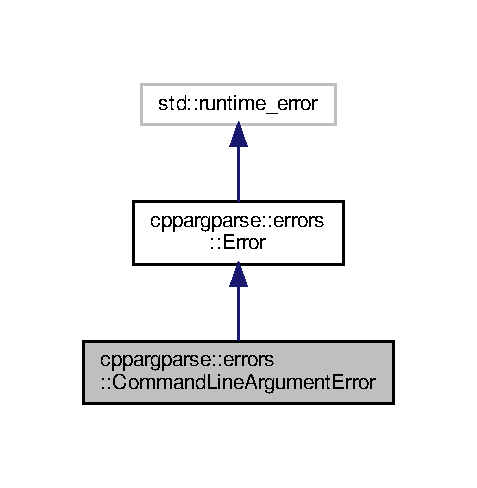
\includegraphics[width=229pt]{classcppargparse_1_1errors_1_1CommandLineArgumentError__inherit__graph}
\end{center}
\end{figure}


Collaboration diagram for cppargparse\+:\+:errors\+:\+:Command\+Line\+Argument\+Error\+:
\nopagebreak
\begin{figure}[H]
\begin{center}
\leavevmode
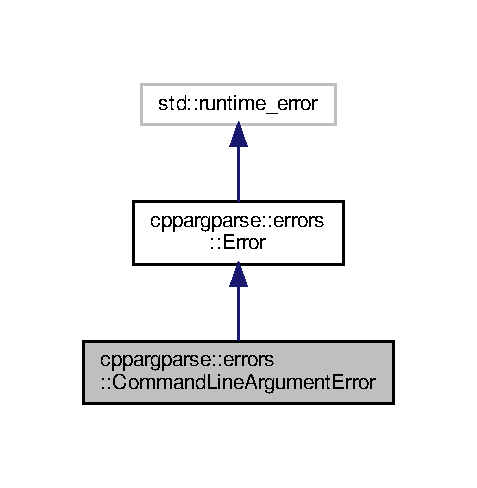
\includegraphics[width=229pt]{classcppargparse_1_1errors_1_1CommandLineArgumentError__coll__graph}
\end{center}
\end{figure}
\subsection*{Public Member Functions}
\begin{DoxyCompactItemize}
\item 
\hyperlink{classcppargparse_1_1errors_1_1CommandLineArgumentError_acb14010d573ba078332a149d2ebf3be6}{Command\+Line\+Argument\+Error} (const std\+::string \&message)
\begin{DoxyCompactList}\small\item\em c\textquotesingle{}tor \end{DoxyCompactList}\end{DoxyCompactItemize}


\subsection{Detailed Description}
\hyperlink{classcppargparse_1_1errors_1_1Error}{Error} class for command line argument errors. 

\subsection{Constructor \& Destructor Documentation}
\mbox{\Hypertarget{classcppargparse_1_1errors_1_1CommandLineArgumentError_acb14010d573ba078332a149d2ebf3be6}\label{classcppargparse_1_1errors_1_1CommandLineArgumentError_acb14010d573ba078332a149d2ebf3be6}} 
\index{cppargparse\+::errors\+::\+Command\+Line\+Argument\+Error@{cppargparse\+::errors\+::\+Command\+Line\+Argument\+Error}!Command\+Line\+Argument\+Error@{Command\+Line\+Argument\+Error}}
\index{Command\+Line\+Argument\+Error@{Command\+Line\+Argument\+Error}!cppargparse\+::errors\+::\+Command\+Line\+Argument\+Error@{cppargparse\+::errors\+::\+Command\+Line\+Argument\+Error}}
\subsubsection{\texorpdfstring{Command\+Line\+Argument\+Error()}{CommandLineArgumentError()}}
{\footnotesize\ttfamily cppargparse\+::errors\+::\+Command\+Line\+Argument\+Error\+::\+Command\+Line\+Argument\+Error (\begin{DoxyParamCaption}\item[{const std\+::string \&}]{message }\end{DoxyParamCaption})\hspace{0.3cm}{\ttfamily [inline]}, {\ttfamily [explicit]}}



c\textquotesingle{}tor 


\begin{DoxyParams}{Parameters}
{\em message} & The error message. \\
\hline
\end{DoxyParams}


The documentation for this class was generated from the following file\+:\begin{DoxyCompactItemize}
\item 
include/cppargparse/errors.\+h\end{DoxyCompactItemize}

\hypertarget{classcppargparse_1_1errors_1_1CommandLineOptionError}{}\section{cppargparse\+:\+:errors\+:\+:Command\+Line\+Option\+Error Class Reference}
\label{classcppargparse_1_1errors_1_1CommandLineOptionError}\index{cppargparse\+::errors\+::\+Command\+Line\+Option\+Error@{cppargparse\+::errors\+::\+Command\+Line\+Option\+Error}}


\hyperlink{classcppargparse_1_1errors_1_1Error}{Error} class for command line option errors.  




{\ttfamily \#include $<$errors.\+h$>$}



Inheritance diagram for cppargparse\+:\+:errors\+:\+:Command\+Line\+Option\+Error\+:
\nopagebreak
\begin{figure}[H]
\begin{center}
\leavevmode
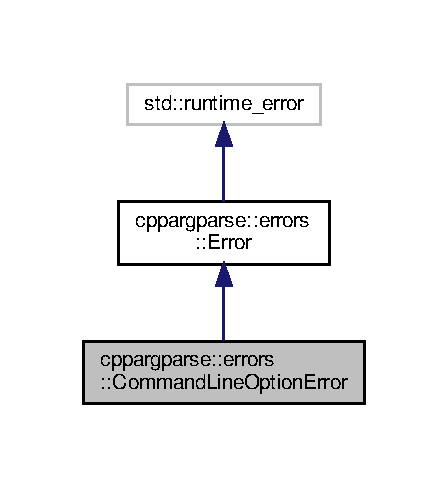
\includegraphics[width=215pt]{classcppargparse_1_1errors_1_1CommandLineOptionError__inherit__graph}
\end{center}
\end{figure}


Collaboration diagram for cppargparse\+:\+:errors\+:\+:Command\+Line\+Option\+Error\+:
\nopagebreak
\begin{figure}[H]
\begin{center}
\leavevmode
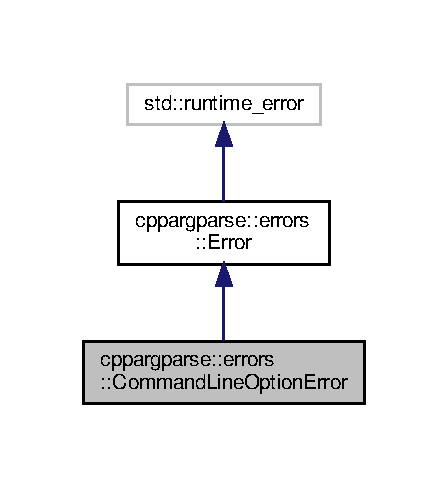
\includegraphics[width=215pt]{classcppargparse_1_1errors_1_1CommandLineOptionError__coll__graph}
\end{center}
\end{figure}
\subsection*{Public Member Functions}
\begin{DoxyCompactItemize}
\item 
\hyperlink{classcppargparse_1_1errors_1_1CommandLineOptionError_a587934b01bd577262174bd82af79b75c}{Command\+Line\+Option\+Error} (const std\+::string \&message)
\begin{DoxyCompactList}\small\item\em c\textquotesingle{}tor \end{DoxyCompactList}\end{DoxyCompactItemize}


\subsection{Detailed Description}
\hyperlink{classcppargparse_1_1errors_1_1Error}{Error} class for command line option errors. 

\subsection{Constructor \& Destructor Documentation}
\mbox{\Hypertarget{classcppargparse_1_1errors_1_1CommandLineOptionError_a587934b01bd577262174bd82af79b75c}\label{classcppargparse_1_1errors_1_1CommandLineOptionError_a587934b01bd577262174bd82af79b75c}} 
\index{cppargparse\+::errors\+::\+Command\+Line\+Option\+Error@{cppargparse\+::errors\+::\+Command\+Line\+Option\+Error}!Command\+Line\+Option\+Error@{Command\+Line\+Option\+Error}}
\index{Command\+Line\+Option\+Error@{Command\+Line\+Option\+Error}!cppargparse\+::errors\+::\+Command\+Line\+Option\+Error@{cppargparse\+::errors\+::\+Command\+Line\+Option\+Error}}
\subsubsection{\texorpdfstring{Command\+Line\+Option\+Error()}{CommandLineOptionError()}}
{\footnotesize\ttfamily cppargparse\+::errors\+::\+Command\+Line\+Option\+Error\+::\+Command\+Line\+Option\+Error (\begin{DoxyParamCaption}\item[{const std\+::string \&}]{message }\end{DoxyParamCaption})\hspace{0.3cm}{\ttfamily [inline]}, {\ttfamily [explicit]}}



c\textquotesingle{}tor 


\begin{DoxyParams}{Parameters}
{\em message} & The error message. \\
\hline
\end{DoxyParams}


The documentation for this class was generated from the following file\+:\begin{DoxyCompactItemize}
\item 
include/cppargparse/errors.\+h\end{DoxyCompactItemize}

\hypertarget{classcppargparse_1_1errors_1_1Error}{}\section{cppargparse\+:\+:errors\+:\+:Error Class Reference}
\label{classcppargparse_1_1errors_1_1Error}\index{cppargparse\+::errors\+::\+Error@{cppargparse\+::errors\+::\+Error}}


Base error class.  




{\ttfamily \#include $<$errors.\+h$>$}



Inheritance diagram for cppargparse\+:\+:errors\+:\+:Error\+:
\nopagebreak
\begin{figure}[H]
\begin{center}
\leavevmode
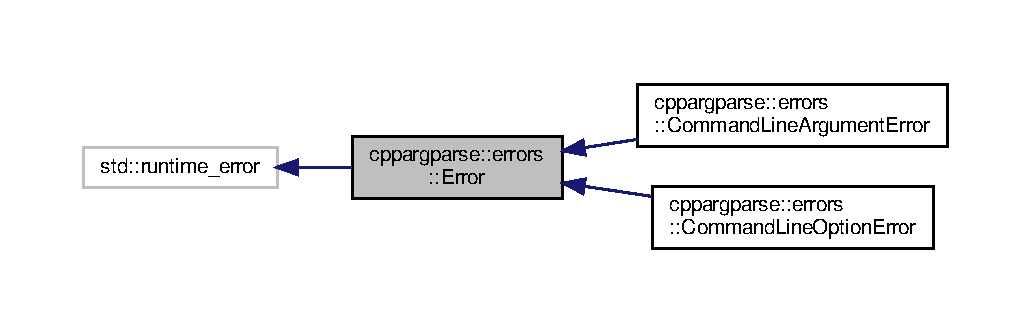
\includegraphics[width=350pt]{classcppargparse_1_1errors_1_1Error__inherit__graph}
\end{center}
\end{figure}


Collaboration diagram for cppargparse\+:\+:errors\+:\+:Error\+:
\nopagebreak
\begin{figure}[H]
\begin{center}
\leavevmode
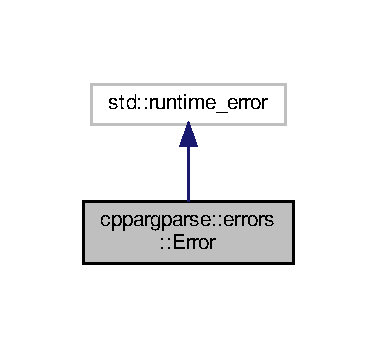
\includegraphics[width=181pt]{classcppargparse_1_1errors_1_1Error__coll__graph}
\end{center}
\end{figure}
\subsection*{Public Member Functions}
\begin{DoxyCompactItemize}
\item 
\hyperlink{classcppargparse_1_1errors_1_1Error_a41c12888d001504fbaec210c5574b91a}{Error} (const std\+::string \&message)
\begin{DoxyCompactList}\small\item\em c\textquotesingle{}tor \end{DoxyCompactList}\end{DoxyCompactItemize}


\subsection{Detailed Description}
Base error class. 

\subsection{Constructor \& Destructor Documentation}
\mbox{\Hypertarget{classcppargparse_1_1errors_1_1Error_a41c12888d001504fbaec210c5574b91a}\label{classcppargparse_1_1errors_1_1Error_a41c12888d001504fbaec210c5574b91a}} 
\index{cppargparse\+::errors\+::\+Error@{cppargparse\+::errors\+::\+Error}!Error@{Error}}
\index{Error@{Error}!cppargparse\+::errors\+::\+Error@{cppargparse\+::errors\+::\+Error}}
\subsubsection{\texorpdfstring{Error()}{Error()}}
{\footnotesize\ttfamily cppargparse\+::errors\+::\+Error\+::\+Error (\begin{DoxyParamCaption}\item[{const std\+::string \&}]{message }\end{DoxyParamCaption})\hspace{0.3cm}{\ttfamily [inline]}, {\ttfamily [explicit]}}



c\textquotesingle{}tor 


\begin{DoxyParams}{Parameters}
{\em message} & The error message. \\
\hline
\end{DoxyParams}


The documentation for this class was generated from the following file\+:\begin{DoxyCompactItemize}
\item 
include/cppargparse/errors.\+h\end{DoxyCompactItemize}

\chapter{File Documentation}
\hypertarget{algorithm_8h}{}\section{include/cppargparse/algorithm.h File Reference}
\label{algorithm_8h}\index{include/cppargparse/algorithm.\+h@{include/cppargparse/algorithm.\+h}}


Static command line related algorithm functions.  


{\ttfamily \#include $<$algorithm$>$}\newline
{\ttfamily \#include \char`\"{}types.\+h\char`\"{}}\newline
Include dependency graph for algorithm.\+h\+:\nopagebreak
\begin{figure}[H]
\begin{center}
\leavevmode
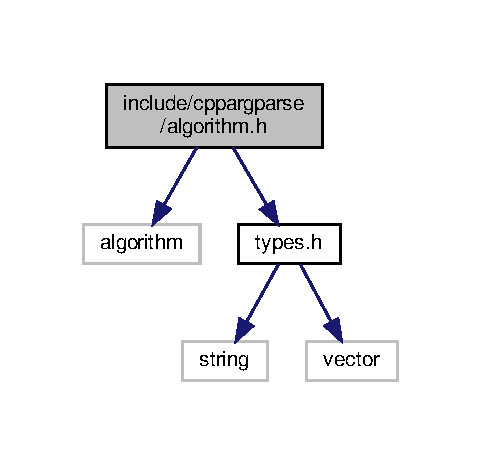
\includegraphics[width=231pt]{algorithm_8h__incl}
\end{center}
\end{figure}
This graph shows which files directly or indirectly include this file\+:\nopagebreak
\begin{figure}[H]
\begin{center}
\leavevmode
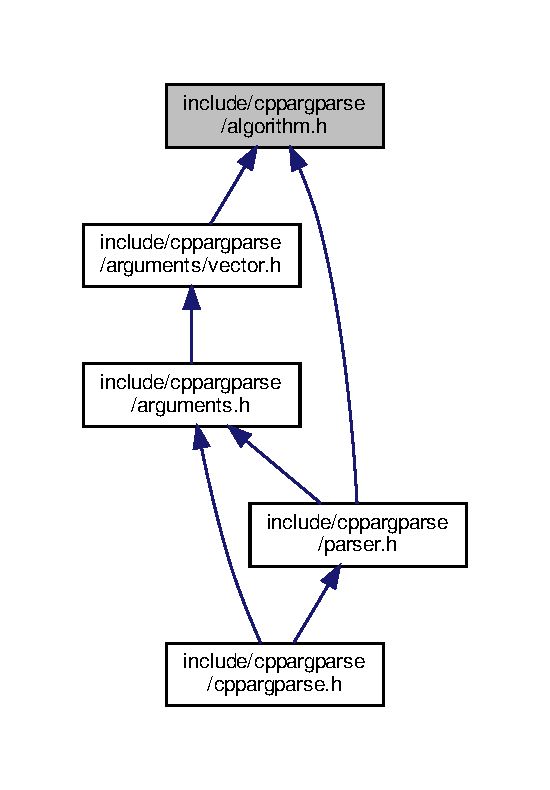
\includegraphics[width=264pt]{algorithm_8h__dep__incl}
\end{center}
\end{figure}
\subsection*{Functions}
\begin{DoxyCompactItemize}
\item 
types\+::\+Command\+Line\+Argument\+Position\+\_\+t \hyperlink{algorithm_8h_aacd4544d12e2d7aad474f25398abab6a}{cppargparse\+::algorithm\+::find\+\_\+arg} (const types\+::\+Command\+Line\+Arguments\+\_\+t \&cmdargs, const std\+::string \&id)
\begin{DoxyCompactList}\small\item\em Find an argument by its ID. \end{DoxyCompactList}\item 
types\+::\+Command\+Line\+Position\+\_\+t \hyperlink{algorithm_8h_ade27151f3d496105c5924c81cdac3ca8}{cppargparse\+::algorithm\+::find\+\_\+arg\+\_\+position} (const types\+::\+Command\+Line\+\_\+t \&cmd, const std\+::string \&id, const std\+::string \&id\+\_\+alt)
\begin{DoxyCompactList}\small\item\em Find an argument\textquotesingle{}s command line position by its ID. \end{DoxyCompactList}\end{DoxyCompactItemize}


\subsection{Detailed Description}
Static command line related algorithm functions. 



\subsection{Function Documentation}
\mbox{\Hypertarget{algorithm_8h_file_aacd4544d12e2d7aad474f25398abab6a}\label{algorithm_8h_file_aacd4544d12e2d7aad474f25398abab6a}} 
\index{algorithm.\+h@{algorithm.\+h}!find\+\_\+arg@{find\+\_\+arg}}
\index{find\+\_\+arg@{find\+\_\+arg}!algorithm.\+h@{algorithm.\+h}}
\subsubsection{\texorpdfstring{find\+\_\+arg()}{find\_arg()}}
{\footnotesize\ttfamily types\+::\+Command\+Line\+Argument\+Position\+\_\+t cppargparse\+::algorithm\+::find\+\_\+arg (\begin{DoxyParamCaption}\item[{const \hyperlink{types_8h_a003c660afe2ee9c6cc39aea966e8926d}{types\+::\+Command\+Line\+Arguments\+\_\+t} \&}]{cmdargs,  }\item[{const std\+::string \&}]{id }\end{DoxyParamCaption})}



Find an argument by its ID. 


\begin{DoxyParams}{Parameters}
{\em cmdargs} & The command line arguments to lookup the argument ID. \\
\hline
{\em id} & The argument ID. Can also be the argument\textquotesingle{}s alterinative ID.\\
\hline
\end{DoxyParams}
\begin{DoxyReturn}{Returns}
The command line arguments iterator position of the argument. 
\end{DoxyReturn}
\mbox{\Hypertarget{algorithm_8h_file_ade27151f3d496105c5924c81cdac3ca8}\label{algorithm_8h_file_ade27151f3d496105c5924c81cdac3ca8}} 
\index{algorithm.\+h@{algorithm.\+h}!find\+\_\+arg\+\_\+position@{find\+\_\+arg\+\_\+position}}
\index{find\+\_\+arg\+\_\+position@{find\+\_\+arg\+\_\+position}!algorithm.\+h@{algorithm.\+h}}
\subsubsection{\texorpdfstring{find\+\_\+arg\+\_\+position()}{find\_arg\_position()}}
{\footnotesize\ttfamily types\+::\+Command\+Line\+Position\+\_\+t cppargparse\+::algorithm\+::find\+\_\+arg\+\_\+position (\begin{DoxyParamCaption}\item[{const \hyperlink{types_8h_a80adf2418b7ce9fe616698efa7533ecf}{types\+::\+Command\+Line\+\_\+t} \&}]{cmd,  }\item[{const std\+::string \&}]{id,  }\item[{const std\+::string \&}]{id\+\_\+alt }\end{DoxyParamCaption})}



Find an argument\textquotesingle{}s command line position by its ID. 


\begin{DoxyParams}{Parameters}
{\em cmd} & The command line. \\
\hline
{\em id} & The argument ID. \\
\hline
{\em id\+\_\+alt} & The argument alternative ID.\\
\hline
\end{DoxyParams}
\begin{DoxyReturn}{Returns}
The command line iterator position of the argument. 
\end{DoxyReturn}

\hypertarget{arguments_8h}{}\section{include/cppargparse/arguments.h File Reference}
\label{arguments_8h}\index{include/cppargparse/arguments.\+h@{include/cppargparse/arguments.\+h}}


Shorthand for including all builtin type converters.  


{\ttfamily \#include $<$cppargparse/arguments/default.\+h$>$}\newline
{\ttfamily \#include $<$cppargparse/arguments/double.\+h$>$}\newline
{\ttfamily \#include $<$cppargparse/arguments/float.\+h$>$}\newline
{\ttfamily \#include $<$cppargparse/arguments/int.\+h$>$}\newline
{\ttfamily \#include $<$cppargparse/arguments/long.\+h$>$}\newline
{\ttfamily \#include $<$cppargparse/arguments/string.\+h$>$}\newline
{\ttfamily \#include $<$cppargparse/arguments/vector.\+h$>$}\newline
Include dependency graph for arguments.\+h\+:\nopagebreak
\begin{figure}[H]
\begin{center}
\leavevmode
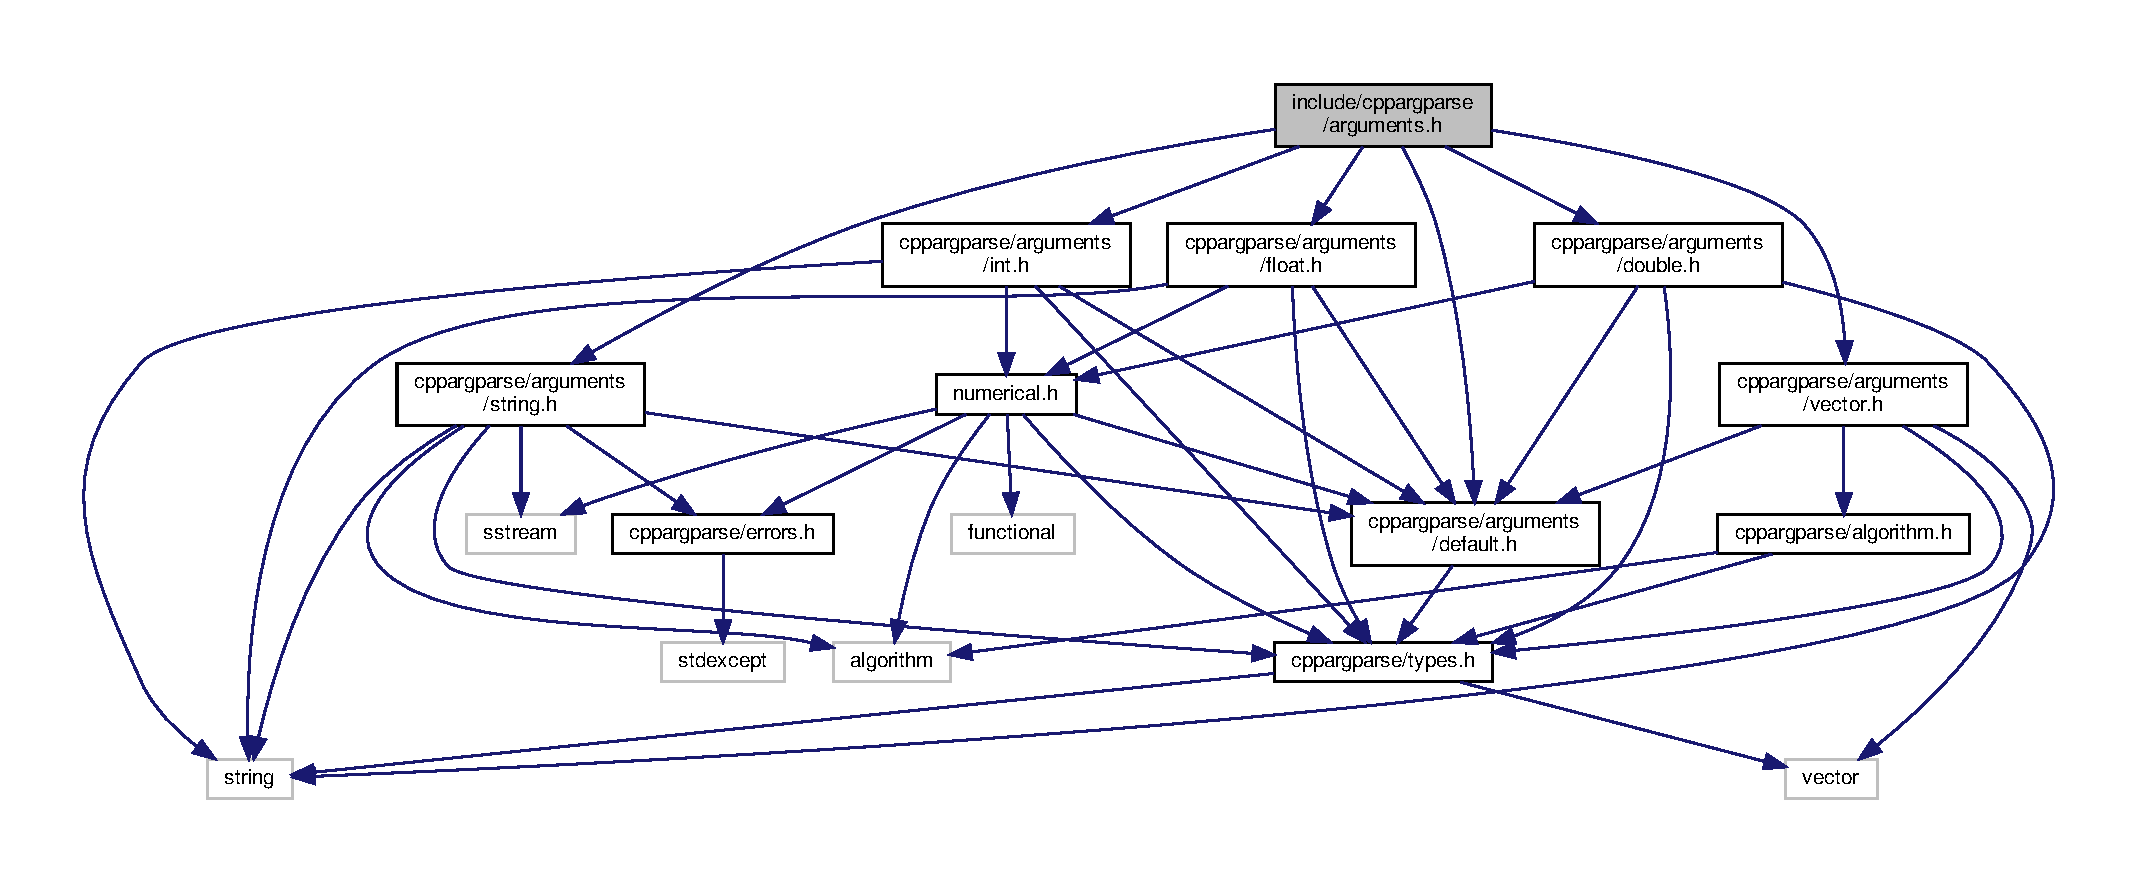
\includegraphics[width=350pt]{arguments_8h__incl}
\end{center}
\end{figure}
This graph shows which files directly or indirectly include this file\+:\nopagebreak
\begin{figure}[H]
\begin{center}
\leavevmode
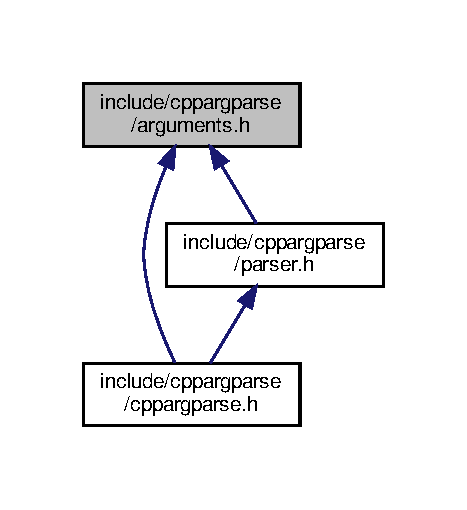
\includegraphics[width=224pt]{arguments_8h__dep__incl}
\end{center}
\end{figure}


\subsection{Detailed Description}
Shorthand for including all builtin type converters. 


\hypertarget{numerical_8h}{}\section{include/cppargparse/arguments/numerical.h File Reference}
\label{numerical_8h}\index{include/cppargparse/arguments/numerical.\+h@{include/cppargparse/arguments/numerical.\+h}}


Static numerical conversion function helpers.  


{\ttfamily \#include $<$algorithm$>$}\newline
{\ttfamily \#include $<$functional$>$}\newline
{\ttfamily \#include $<$sstream$>$}\newline
{\ttfamily \#include $<$cppargparse/errors.\+h$>$}\newline
{\ttfamily \#include $<$cppargparse/types.\+h$>$}\newline
{\ttfamily \#include \char`\"{}default.\+h\char`\"{}}\newline
Include dependency graph for numerical.\+h\+:\nopagebreak
\begin{figure}[H]
\begin{center}
\leavevmode
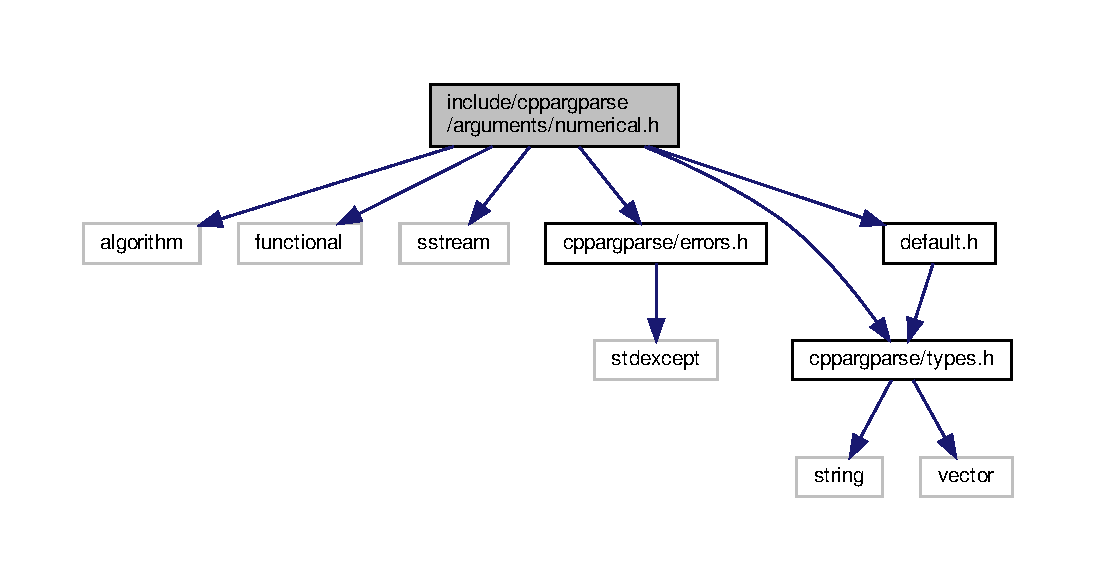
\includegraphics[width=350pt]{numerical_8h__incl}
\end{center}
\end{figure}
This graph shows which files directly or indirectly include this file\+:\nopagebreak
\begin{figure}[H]
\begin{center}
\leavevmode
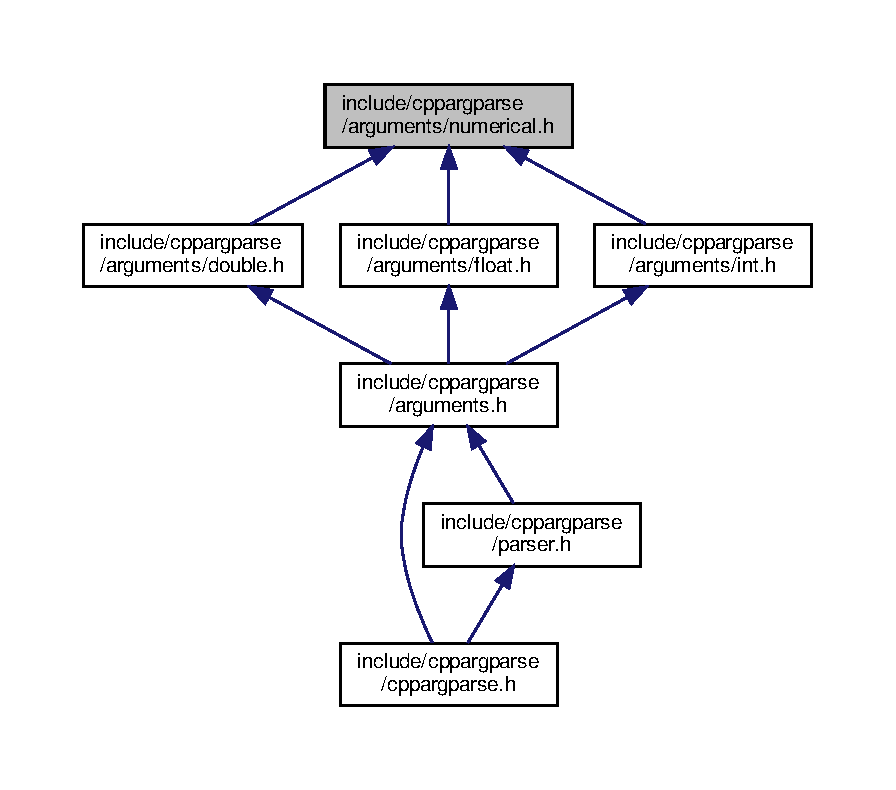
\includegraphics[width=350pt]{numerical_8h__dep__incl}
\end{center}
\end{figure}
\subsection*{Macros}
\begin{DoxyCompactItemize}
\item 
\#define {\bfseries C\+P\+P\+A\+R\+G\+P\+A\+R\+S\+E\+\_\+\+N\+U\+M\+E\+R\+I\+C\+A\+L\+\_\+\+A\+R\+G\+U\+M\+E\+N\+T\+\_\+\+C\+O\+N\+V\+E\+R\+T\+E\+R\+\_\+\+R\+E\+T\+U\+R\+NS}(...)
\item 
\#define {\bfseries C\+P\+P\+A\+R\+G\+P\+A\+R\+S\+E\+\_\+\+N\+U\+M\+E\+R\+I\+C\+A\+L\+\_\+\+A\+R\+G\+U\+M\+E\+N\+T\+\_\+\+C\+O\+N\+V\+E\+R\+T\+E\+R\+\_\+\+O\+V\+E\+R\+L\+O\+A\+DS}(...)
\end{DoxyCompactItemize}


\subsection{Detailed Description}
Static numerical conversion function helpers. 



\subsection{Macro Definition Documentation}
\mbox{\Hypertarget{numerical_8h_a11ac71e245a159e139de4854e5eae730}\label{numerical_8h_a11ac71e245a159e139de4854e5eae730}} 
\index{numerical.\+h@{numerical.\+h}!C\+P\+P\+A\+R\+G\+P\+A\+R\+S\+E\+\_\+\+N\+U\+M\+E\+R\+I\+C\+A\+L\+\_\+\+A\+R\+G\+U\+M\+E\+N\+T\+\_\+\+C\+O\+N\+V\+E\+R\+T\+E\+R\+\_\+\+O\+V\+E\+R\+L\+O\+A\+DS@{C\+P\+P\+A\+R\+G\+P\+A\+R\+S\+E\+\_\+\+N\+U\+M\+E\+R\+I\+C\+A\+L\+\_\+\+A\+R\+G\+U\+M\+E\+N\+T\+\_\+\+C\+O\+N\+V\+E\+R\+T\+E\+R\+\_\+\+O\+V\+E\+R\+L\+O\+A\+DS}}
\index{C\+P\+P\+A\+R\+G\+P\+A\+R\+S\+E\+\_\+\+N\+U\+M\+E\+R\+I\+C\+A\+L\+\_\+\+A\+R\+G\+U\+M\+E\+N\+T\+\_\+\+C\+O\+N\+V\+E\+R\+T\+E\+R\+\_\+\+O\+V\+E\+R\+L\+O\+A\+DS@{C\+P\+P\+A\+R\+G\+P\+A\+R\+S\+E\+\_\+\+N\+U\+M\+E\+R\+I\+C\+A\+L\+\_\+\+A\+R\+G\+U\+M\+E\+N\+T\+\_\+\+C\+O\+N\+V\+E\+R\+T\+E\+R\+\_\+\+O\+V\+E\+R\+L\+O\+A\+DS}!numerical.\+h@{numerical.\+h}}
\subsubsection{\texorpdfstring{C\+P\+P\+A\+R\+G\+P\+A\+R\+S\+E\+\_\+\+N\+U\+M\+E\+R\+I\+C\+A\+L\+\_\+\+A\+R\+G\+U\+M\+E\+N\+T\+\_\+\+C\+O\+N\+V\+E\+R\+T\+E\+R\+\_\+\+O\+V\+E\+R\+L\+O\+A\+DS}{CPPARGPARSE\_NUMERICAL\_ARGUMENT\_CONVERTER\_OVERLOADS}}
{\footnotesize\ttfamily \#define C\+P\+P\+A\+R\+G\+P\+A\+R\+S\+E\+\_\+\+N\+U\+M\+E\+R\+I\+C\+A\+L\+\_\+\+A\+R\+G\+U\+M\+E\+N\+T\+\_\+\+C\+O\+N\+V\+E\+R\+T\+E\+R\+\_\+\+O\+V\+E\+R\+L\+O\+A\+DS(\begin{DoxyParamCaption}\item[{}]{... }\end{DoxyParamCaption})}

{\bfseries Value\+:}
\begin{DoxyCode}
[](\textcolor{keyword}{auto}&&...args) \(\backslash\)
  CPPARGPARSE\_NUMERICAL\_ARGUMENT\_CONVERTER\_RETURNS( \_\_VA\_ARGS\_\_( decltype(args)(args)... ))
\end{DoxyCode}
\mbox{\Hypertarget{numerical_8h_af3804cc4f013121303678b5315b77f8c}\label{numerical_8h_af3804cc4f013121303678b5315b77f8c}} 
\index{numerical.\+h@{numerical.\+h}!C\+P\+P\+A\+R\+G\+P\+A\+R\+S\+E\+\_\+\+N\+U\+M\+E\+R\+I\+C\+A\+L\+\_\+\+A\+R\+G\+U\+M\+E\+N\+T\+\_\+\+C\+O\+N\+V\+E\+R\+T\+E\+R\+\_\+\+R\+E\+T\+U\+R\+NS@{C\+P\+P\+A\+R\+G\+P\+A\+R\+S\+E\+\_\+\+N\+U\+M\+E\+R\+I\+C\+A\+L\+\_\+\+A\+R\+G\+U\+M\+E\+N\+T\+\_\+\+C\+O\+N\+V\+E\+R\+T\+E\+R\+\_\+\+R\+E\+T\+U\+R\+NS}}
\index{C\+P\+P\+A\+R\+G\+P\+A\+R\+S\+E\+\_\+\+N\+U\+M\+E\+R\+I\+C\+A\+L\+\_\+\+A\+R\+G\+U\+M\+E\+N\+T\+\_\+\+C\+O\+N\+V\+E\+R\+T\+E\+R\+\_\+\+R\+E\+T\+U\+R\+NS@{C\+P\+P\+A\+R\+G\+P\+A\+R\+S\+E\+\_\+\+N\+U\+M\+E\+R\+I\+C\+A\+L\+\_\+\+A\+R\+G\+U\+M\+E\+N\+T\+\_\+\+C\+O\+N\+V\+E\+R\+T\+E\+R\+\_\+\+R\+E\+T\+U\+R\+NS}!numerical.\+h@{numerical.\+h}}
\subsubsection{\texorpdfstring{C\+P\+P\+A\+R\+G\+P\+A\+R\+S\+E\+\_\+\+N\+U\+M\+E\+R\+I\+C\+A\+L\+\_\+\+A\+R\+G\+U\+M\+E\+N\+T\+\_\+\+C\+O\+N\+V\+E\+R\+T\+E\+R\+\_\+\+R\+E\+T\+U\+R\+NS}{CPPARGPARSE\_NUMERICAL\_ARGUMENT\_CONVERTER\_RETURNS}}
{\footnotesize\ttfamily \#define C\+P\+P\+A\+R\+G\+P\+A\+R\+S\+E\+\_\+\+N\+U\+M\+E\+R\+I\+C\+A\+L\+\_\+\+A\+R\+G\+U\+M\+E\+N\+T\+\_\+\+C\+O\+N\+V\+E\+R\+T\+E\+R\+\_\+\+R\+E\+T\+U\+R\+NS(\begin{DoxyParamCaption}\item[{}]{... }\end{DoxyParamCaption})}

{\bfseries Value\+:}
\begin{DoxyCode}
noexcept(noexcept(\_\_VA\_ARGS\_\_)) \(\backslash\)
  -> decltype( \_\_VA\_ARGS\_\_ ) \(\backslash\)
  \{ \textcolor{keywordflow}{return} \_\_VA\_ARGS\_\_; \}
\end{DoxyCode}

\hypertarget{cppargparse_8h}{}\section{include/cppargparse/cppargparse.h File Reference}
\label{cppargparse_8h}\index{include/cppargparse/cppargparse.\+h@{include/cppargparse/cppargparse.\+h}}


Shorthand for including the whole library at once.  


{\ttfamily \#include $<$cppargparse/types.\+h$>$}\newline
{\ttfamily \#include $<$cppargparse/arguments.\+h$>$}\newline
{\ttfamily \#include $<$cppargparse/parser/parser.\+h$>$}\newline
{\ttfamily \#include $<$cppargparse/errors.\+h$>$}\newline
Include dependency graph for cppargparse.\+h\+:\nopagebreak
\begin{figure}[H]
\begin{center}
\leavevmode
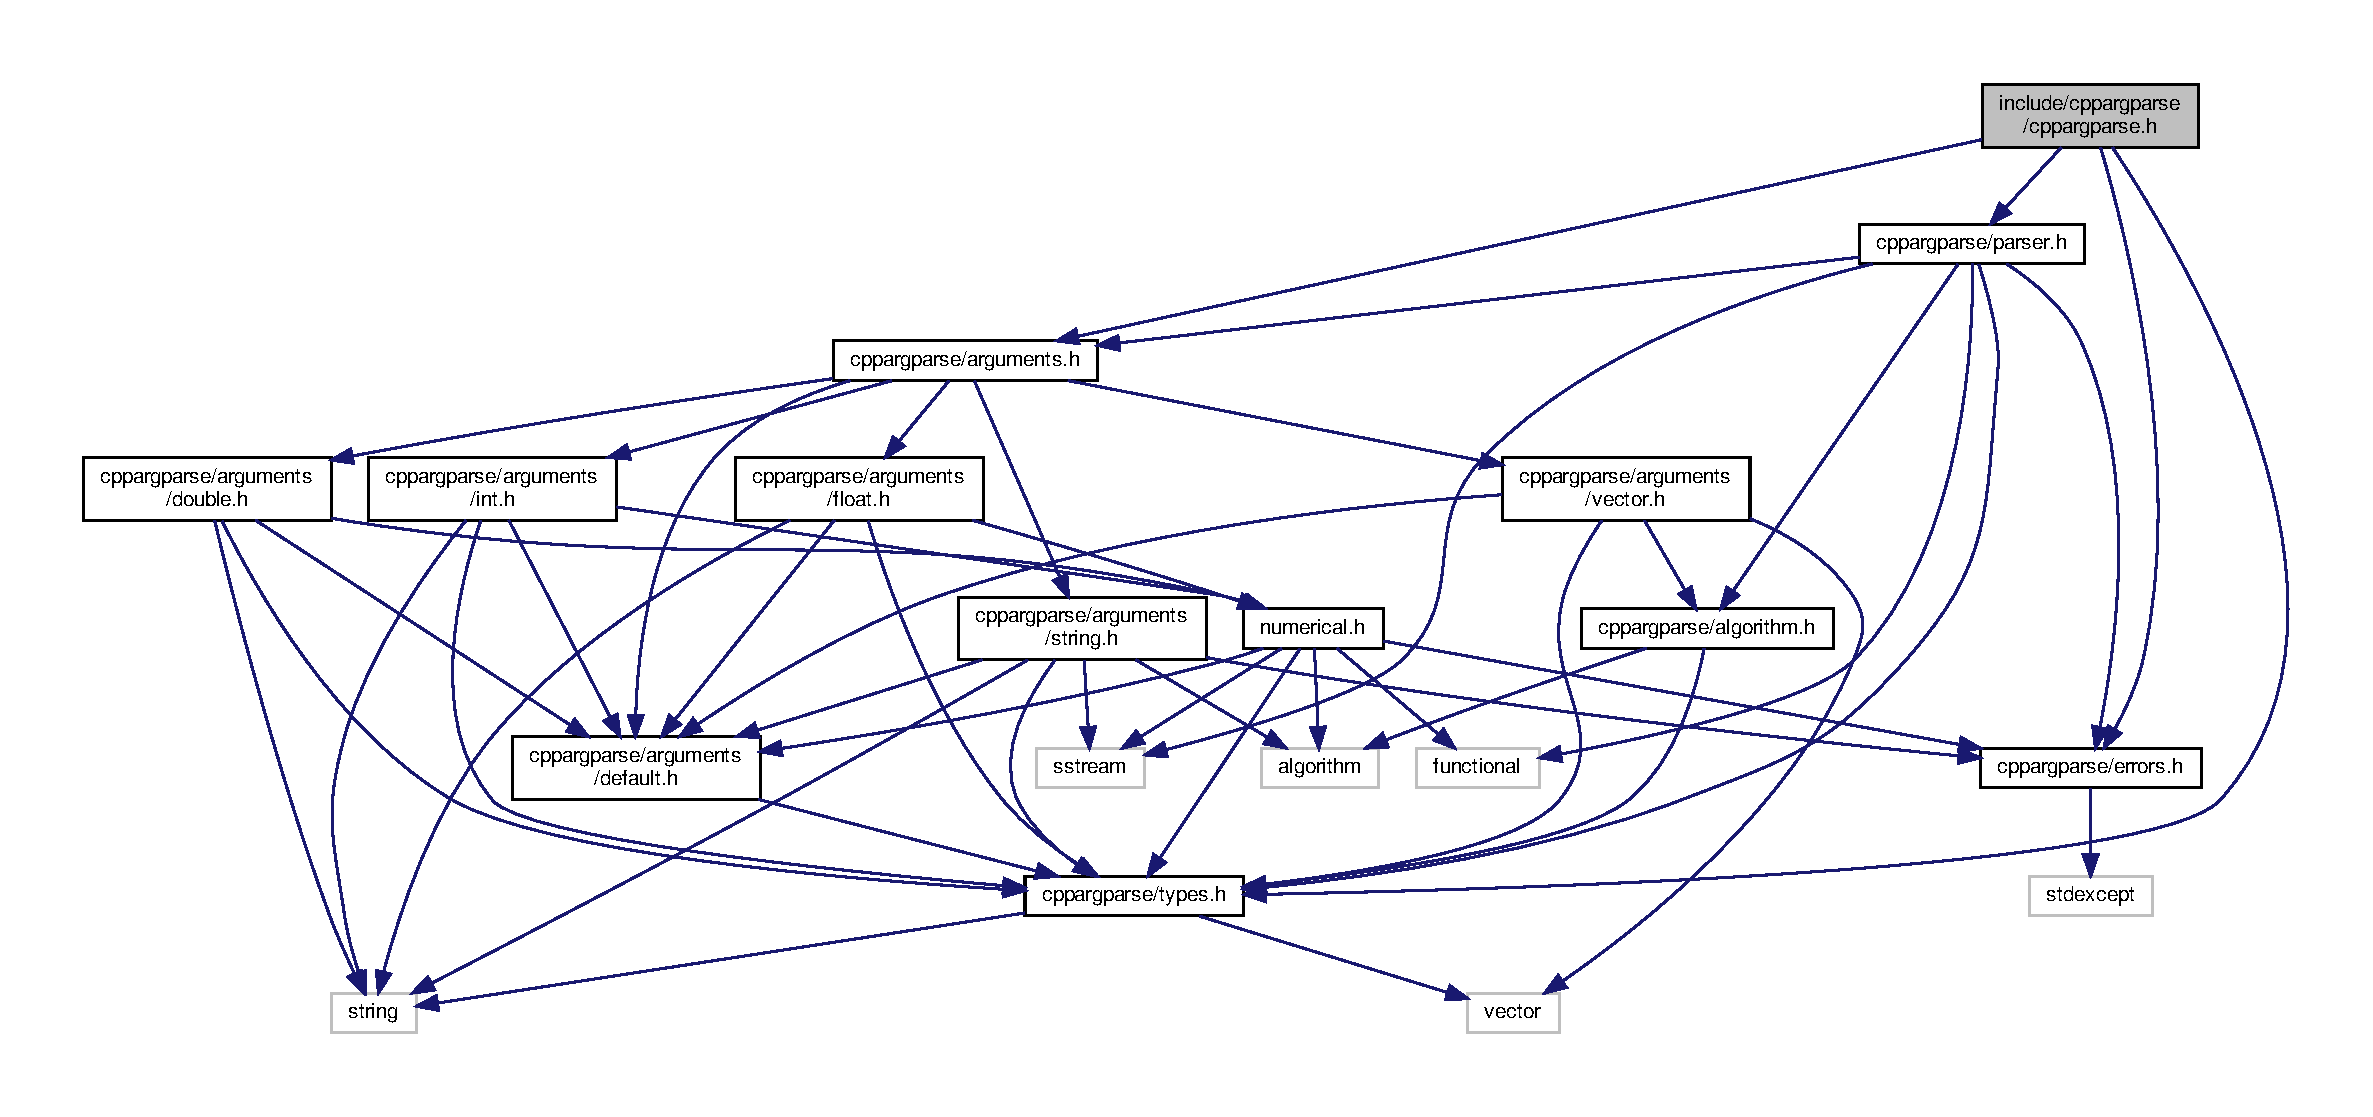
\includegraphics[width=350pt]{cppargparse_8h__incl}
\end{center}
\end{figure}


\subsection{Detailed Description}
Shorthand for including the whole library at once. 


\hypertarget{types_8h}{}\section{include/cppargparse/types.h File Reference}
\label{types_8h}\index{include/cppargparse/types.\+h@{include/cppargparse/types.\+h}}


Global type definitions of command line related types.  


{\ttfamily \#include $<$string$>$}\newline
{\ttfamily \#include $<$vector$>$}\newline
Include dependency graph for types.\+h\+:\nopagebreak
\begin{figure}[H]
\begin{center}
\leavevmode
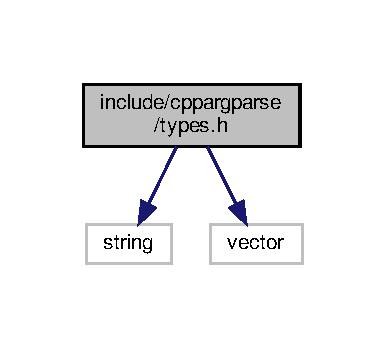
\includegraphics[width=185pt]{types_8h__incl}
\end{center}
\end{figure}
This graph shows which files directly or indirectly include this file\+:\nopagebreak
\begin{figure}[H]
\begin{center}
\leavevmode
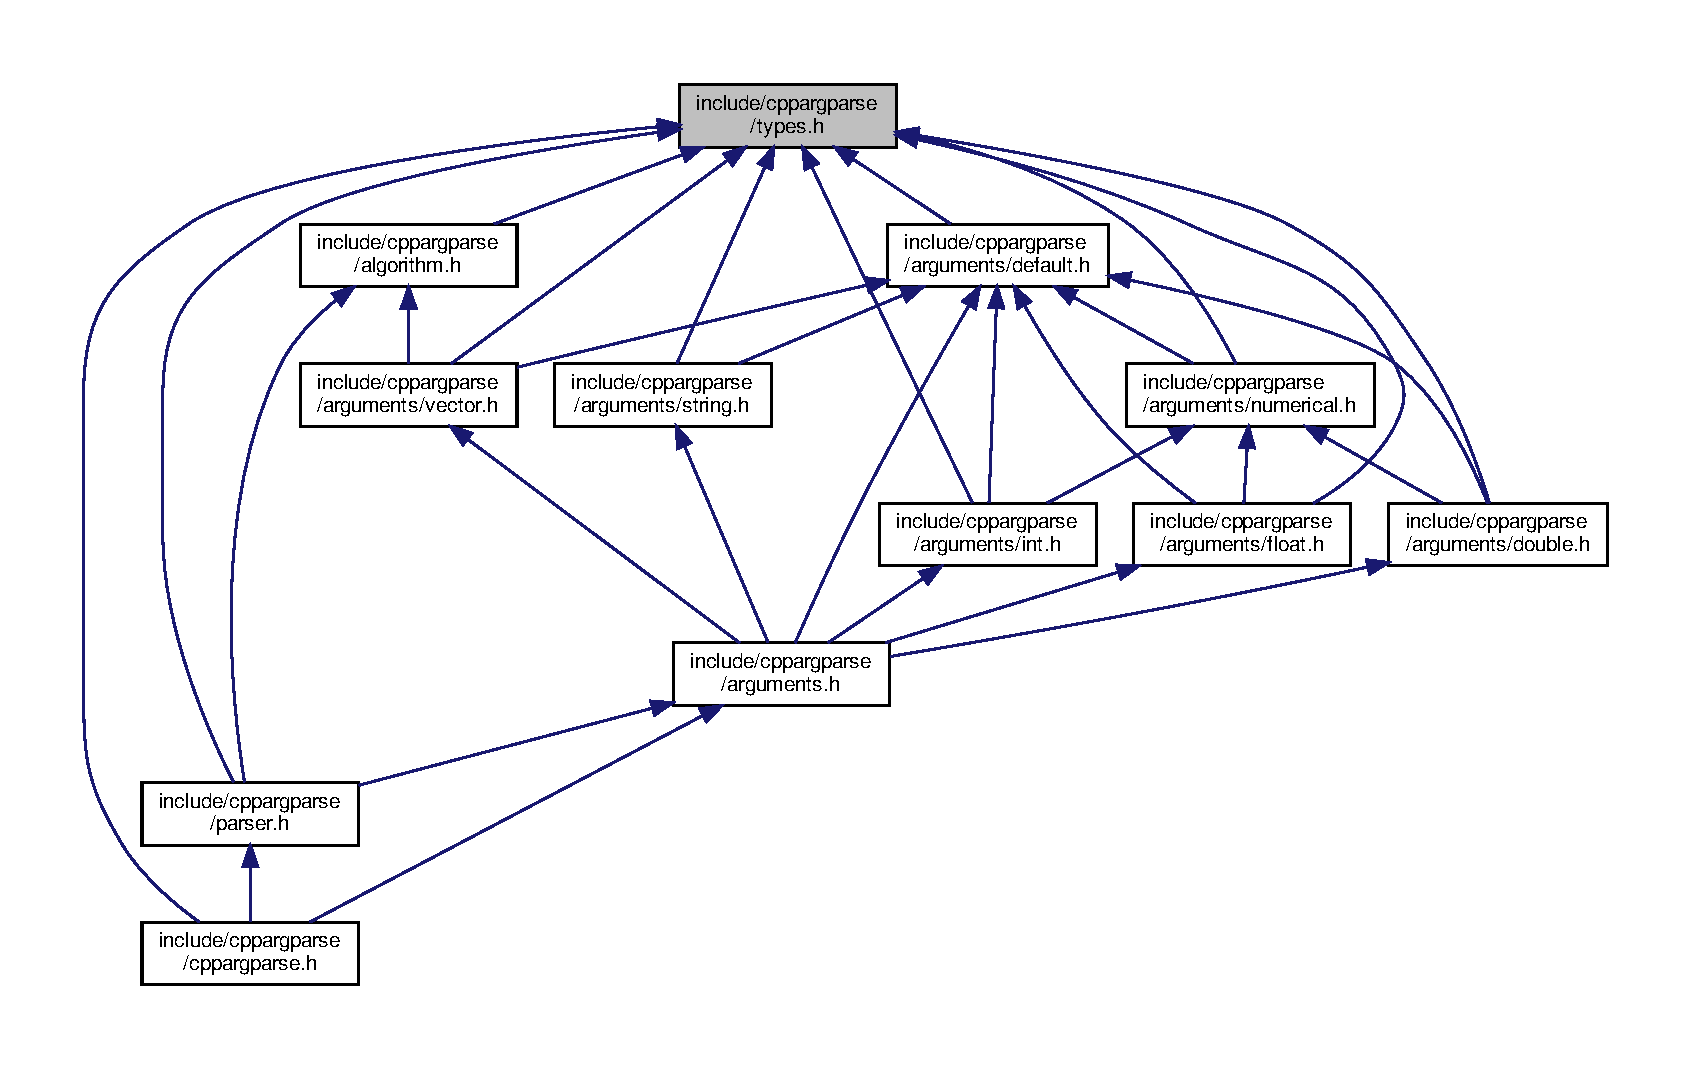
\includegraphics[width=350pt]{types_8h__dep__incl}
\end{center}
\end{figure}
\subsection*{Classes}
\begin{DoxyCompactItemize}
\item 
struct \hyperlink{structcppargparse_1_1types_1_1CommandLineArgument__t}{cppargparse\+::types\+::\+Command\+Line\+Argument\+\_\+t}
\begin{DoxyCompactList}\small\item\em The command line argument struct. \end{DoxyCompactList}\end{DoxyCompactItemize}
\subsection*{Typedefs}
\begin{DoxyCompactItemize}
\item 
typedef std\+::vector$<$ std\+::string $>$ \hyperlink{types_8h_a80adf2418b7ce9fe616698efa7533ecf}{cppargparse\+::types\+::\+Command\+Line\+\_\+t}
\begin{DoxyCompactList}\small\item\em The command line type. \end{DoxyCompactList}\item 
\mbox{\Hypertarget{types_8h_a43b4f43f8940de1bf09ced6f1b668053}\label{types_8h_a43b4f43f8940de1bf09ced6f1b668053}} 
typedef Command\+Line\+\_\+t\+::const\+\_\+iterator \hyperlink{types_8h_a43b4f43f8940de1bf09ced6f1b668053}{cppargparse\+::types\+::\+Command\+Line\+Position\+\_\+t}
\begin{DoxyCompactList}\small\item\em The command line iterator position type. \end{DoxyCompactList}\item 
\mbox{\Hypertarget{types_8h_a96efcf8a8929cc8e503e27b180627140}\label{types_8h_a96efcf8a8929cc8e503e27b180627140}} 
typedef std\+::vector$<$ Command\+Line\+Position\+\_\+t $>$ \hyperlink{types_8h_a96efcf8a8929cc8e503e27b180627140}{cppargparse\+::types\+::\+Command\+Line\+Positions\+\_\+t}
\begin{DoxyCompactList}\small\item\em The command line iterator positions type. \end{DoxyCompactList}\item 
\mbox{\Hypertarget{types_8h_a003c660afe2ee9c6cc39aea966e8926d}\label{types_8h_a003c660afe2ee9c6cc39aea966e8926d}} 
typedef std\+::vector$<$ Command\+Line\+Argument\+\_\+t $>$ \hyperlink{types_8h_a003c660afe2ee9c6cc39aea966e8926d}{cppargparse\+::types\+::\+Command\+Line\+Arguments\+\_\+t}
\begin{DoxyCompactList}\small\item\em The command line arguments type. \end{DoxyCompactList}\item 
\mbox{\Hypertarget{types_8h_abbf49636a18c014e5bad6ae4a82bb8bc}\label{types_8h_abbf49636a18c014e5bad6ae4a82bb8bc}} 
typedef Command\+Line\+Arguments\+\_\+t\+::const\+\_\+iterator \hyperlink{types_8h_abbf49636a18c014e5bad6ae4a82bb8bc}{cppargparse\+::types\+::\+Command\+Line\+Argument\+Position\+\_\+t}
\begin{DoxyCompactList}\small\item\em The command line argument iterator position type. \end{DoxyCompactList}\end{DoxyCompactItemize}


\subsection{Detailed Description}
Global type definitions of command line related types. 



\subsection{Typedef Documentation}
\mbox{\Hypertarget{types_8h_file_a80adf2418b7ce9fe616698efa7533ecf}\label{types_8h_file_a80adf2418b7ce9fe616698efa7533ecf}} 
\index{types.\+h@{types.\+h}!Command\+Line\+\_\+t@{Command\+Line\+\_\+t}}
\index{Command\+Line\+\_\+t@{Command\+Line\+\_\+t}!types.\+h@{types.\+h}}
\subsubsection{\texorpdfstring{Command\+Line\+\_\+t}{CommandLine\_t}}
{\footnotesize\ttfamily typedef std\+::vector$<$std\+::string$>$ \hyperlink{types_8h_a80adf2418b7ce9fe616698efa7533ecf}{cppargparse\+::types\+::\+Command\+Line\+\_\+t}}



The command line type. 

Example\+: \char`\"{}-\/t 5 -\/o output.\+txt\char`\"{} 
%--- End generated contents ---

% Index
\backmatter
\newpage
\phantomsection
\clearemptydoublepage
\addcontentsline{toc}{chapter}{Index}
\printindex

\end{document}
